% Options for packages loaded elsewhere
\PassOptionsToPackage{unicode}{hyperref}
\PassOptionsToPackage{hyphens}{url}
%
\documentclass[
]{article}
\usepackage{amsmath,amssymb}
\usepackage{iftex}
\ifPDFTeX
  \usepackage[T1]{fontenc}
  \usepackage[utf8]{inputenc}
  \usepackage{textcomp} % provide euro and other symbols
\else % if luatex or xetex
  \usepackage{unicode-math} % this also loads fontspec
  \defaultfontfeatures{Scale=MatchLowercase}
  \defaultfontfeatures[\rmfamily]{Ligatures=TeX,Scale=1}
\fi
\usepackage{lmodern}
\ifPDFTeX\else
  % xetex/luatex font selection
\fi
% Use upquote if available, for straight quotes in verbatim environments
\IfFileExists{upquote.sty}{\usepackage{upquote}}{}
\IfFileExists{microtype.sty}{% use microtype if available
  \usepackage[]{microtype}
  \UseMicrotypeSet[protrusion]{basicmath} % disable protrusion for tt fonts
}{}
\makeatletter
\@ifundefined{KOMAClassName}{% if non-KOMA class
  \IfFileExists{parskip.sty}{%
    \usepackage{parskip}
  }{% else
    \setlength{\parindent}{0pt}
    \setlength{\parskip}{6pt plus 2pt minus 1pt}}
}{% if KOMA class
  \KOMAoptions{parskip=half}}
\makeatother
\usepackage{xcolor}
\usepackage[margin=1in]{geometry}
\usepackage{color}
\usepackage{fancyvrb}
\newcommand{\VerbBar}{|}
\newcommand{\VERB}{\Verb[commandchars=\\\{\}]}
\DefineVerbatimEnvironment{Highlighting}{Verbatim}{commandchars=\\\{\}}
% Add ',fontsize=\small' for more characters per line
\usepackage{framed}
\definecolor{shadecolor}{RGB}{248,248,248}
\newenvironment{Shaded}{\begin{snugshade}}{\end{snugshade}}
\newcommand{\AlertTok}[1]{\textcolor[rgb]{0.94,0.16,0.16}{#1}}
\newcommand{\AnnotationTok}[1]{\textcolor[rgb]{0.56,0.35,0.01}{\textbf{\textit{#1}}}}
\newcommand{\AttributeTok}[1]{\textcolor[rgb]{0.13,0.29,0.53}{#1}}
\newcommand{\BaseNTok}[1]{\textcolor[rgb]{0.00,0.00,0.81}{#1}}
\newcommand{\BuiltInTok}[1]{#1}
\newcommand{\CharTok}[1]{\textcolor[rgb]{0.31,0.60,0.02}{#1}}
\newcommand{\CommentTok}[1]{\textcolor[rgb]{0.56,0.35,0.01}{\textit{#1}}}
\newcommand{\CommentVarTok}[1]{\textcolor[rgb]{0.56,0.35,0.01}{\textbf{\textit{#1}}}}
\newcommand{\ConstantTok}[1]{\textcolor[rgb]{0.56,0.35,0.01}{#1}}
\newcommand{\ControlFlowTok}[1]{\textcolor[rgb]{0.13,0.29,0.53}{\textbf{#1}}}
\newcommand{\DataTypeTok}[1]{\textcolor[rgb]{0.13,0.29,0.53}{#1}}
\newcommand{\DecValTok}[1]{\textcolor[rgb]{0.00,0.00,0.81}{#1}}
\newcommand{\DocumentationTok}[1]{\textcolor[rgb]{0.56,0.35,0.01}{\textbf{\textit{#1}}}}
\newcommand{\ErrorTok}[1]{\textcolor[rgb]{0.64,0.00,0.00}{\textbf{#1}}}
\newcommand{\ExtensionTok}[1]{#1}
\newcommand{\FloatTok}[1]{\textcolor[rgb]{0.00,0.00,0.81}{#1}}
\newcommand{\FunctionTok}[1]{\textcolor[rgb]{0.13,0.29,0.53}{\textbf{#1}}}
\newcommand{\ImportTok}[1]{#1}
\newcommand{\InformationTok}[1]{\textcolor[rgb]{0.56,0.35,0.01}{\textbf{\textit{#1}}}}
\newcommand{\KeywordTok}[1]{\textcolor[rgb]{0.13,0.29,0.53}{\textbf{#1}}}
\newcommand{\NormalTok}[1]{#1}
\newcommand{\OperatorTok}[1]{\textcolor[rgb]{0.81,0.36,0.00}{\textbf{#1}}}
\newcommand{\OtherTok}[1]{\textcolor[rgb]{0.56,0.35,0.01}{#1}}
\newcommand{\PreprocessorTok}[1]{\textcolor[rgb]{0.56,0.35,0.01}{\textit{#1}}}
\newcommand{\RegionMarkerTok}[1]{#1}
\newcommand{\SpecialCharTok}[1]{\textcolor[rgb]{0.81,0.36,0.00}{\textbf{#1}}}
\newcommand{\SpecialStringTok}[1]{\textcolor[rgb]{0.31,0.60,0.02}{#1}}
\newcommand{\StringTok}[1]{\textcolor[rgb]{0.31,0.60,0.02}{#1}}
\newcommand{\VariableTok}[1]{\textcolor[rgb]{0.00,0.00,0.00}{#1}}
\newcommand{\VerbatimStringTok}[1]{\textcolor[rgb]{0.31,0.60,0.02}{#1}}
\newcommand{\WarningTok}[1]{\textcolor[rgb]{0.56,0.35,0.01}{\textbf{\textit{#1}}}}
\usepackage{longtable,booktabs,array}
\usepackage{calc} % for calculating minipage widths
% Correct order of tables after \paragraph or \subparagraph
\usepackage{etoolbox}
\makeatletter
\patchcmd\longtable{\par}{\if@noskipsec\mbox{}\fi\par}{}{}
\makeatother
% Allow footnotes in longtable head/foot
\IfFileExists{footnotehyper.sty}{\usepackage{footnotehyper}}{\usepackage{footnote}}
\makesavenoteenv{longtable}
\usepackage{graphicx}
\makeatletter
\newsavebox\pandoc@box
\newcommand*\pandocbounded[1]{% scales image to fit in text height/width
  \sbox\pandoc@box{#1}%
  \Gscale@div\@tempa{\textheight}{\dimexpr\ht\pandoc@box+\dp\pandoc@box\relax}%
  \Gscale@div\@tempb{\linewidth}{\wd\pandoc@box}%
  \ifdim\@tempb\p@<\@tempa\p@\let\@tempa\@tempb\fi% select the smaller of both
  \ifdim\@tempa\p@<\p@\scalebox{\@tempa}{\usebox\pandoc@box}%
  \else\usebox{\pandoc@box}%
  \fi%
}
% Set default figure placement to htbp
\def\fps@figure{htbp}
\makeatother
\setlength{\emergencystretch}{3em} % prevent overfull lines
\providecommand{\tightlist}{%
  \setlength{\itemsep}{0pt}\setlength{\parskip}{0pt}}
\setcounter{secnumdepth}{5}
\usepackage{pdfpages}
\usepackage{multirow}
\usepackage{multicol}
\usepackage{colortbl}
\usepackage{hhline}
\newlength\Oldarrayrulewidth
\newlength\Oldtabcolsep
\usepackage{longtable}
\usepackage{array}
\usepackage{hyperref}
\usepackage{float}
\usepackage{wrapfig}
\usepackage{bookmark}
\IfFileExists{xurl.sty}{\usepackage{xurl}}{} % add URL line breaks if available
\urlstyle{same}
\hypersetup{
  pdftitle={Análise de Depressão em Estudantes Indianos},
  hidelinks,
  pdfcreator={LaTeX via pandoc}}

\title{Análise de Depressão em Estudantes Indianos}
\author{Caio Costa Cavalcante\\
Nalanda Xavier da Silva}
\date{16/07/2025}

\begin{document}
\maketitle

{
\setcounter{tocdepth}{2}
\tableofcontents
}
\section{Introdução}\label{introducao}

A saúde mental em ambientes acadêmicos vem recebendo atenção crescente
devido ao aumento dos casos de \textbf{depressão} e \textbf{pensamentos
suicidas} entre estudantes. Este relatório apresenta uma análise
exploratória baseada em um recorte de dados de estudantes universitários
na Índia.

\section{Objetivos}\label{objetivos}

\begin{itemize}
\tightlist
\item
  Estimar a prevalência de depressão e pensamentos suicidas.\\
\item
  Investigar fatores de risco potenciais (pressão acadêmica, duração do
  sono, idade e gênero).\\
\item
  Gerar tabelas e visualizações que possam subsidiar intervenções de
  saúde mental.
\end{itemize}

\section{Fontes de Dados}\label{dados}

\begin{longtable}[]{@{}
  >{\raggedright\arraybackslash}p{(\linewidth - 2\tabcolsep) * \real{0.5000}}
  >{\raggedright\arraybackslash}p{(\linewidth - 2\tabcolsep) * \real{0.5000}}@{}}
\toprule\noalign{}
\begin{minipage}[b]{\linewidth}\raggedright
Origem
\end{minipage} & \begin{minipage}[b]{\linewidth}\raggedright
Link
\end{minipage} \\
\midrule\noalign{}
\endhead
\bottomrule\noalign{}
\endlastfoot
Base derivada usada nesta análise &
\url{https://www.kaggle.com/datasets/ikynahidwin/depression-student-dataset/data} \\
Dataset original completo &
\url{https://www.kaggle.com/datasets/sumansharmadataworld/depression-surveydataset-for-analysis} \\
\end{longtable}

A base \texttt{estudantes\_depressao.csv} presente neste repositório é
um subconjunto limpo e simplificado (≈100 linhas) da fonte acima,
adequado para fins didáticos.

\subsection{Dicionário de
Variáveis}\label{dicionuxe1rio-de-variuxe1veis}

\begin{longtable}[]{@{}
  >{\raggedright\arraybackslash}p{(\linewidth - 4\tabcolsep) * \real{0.3333}}
  >{\raggedright\arraybackslash}p{(\linewidth - 4\tabcolsep) * \real{0.3333}}
  >{\raggedright\arraybackslash}p{(\linewidth - 4\tabcolsep) * \real{0.3333}}@{}}
\toprule\noalign{}
\begin{minipage}[b]{\linewidth}\raggedright
Nome
\end{minipage} & \begin{minipage}[b]{\linewidth}\raggedright
Tipo
\end{minipage} & \begin{minipage}[b]{\linewidth}\raggedright
Descrição
\end{minipage} \\
\midrule\noalign{}
\endhead
\bottomrule\noalign{}
\endlastfoot
\texttt{genero} & \emph{Factor} & Sexo biológico (\texttt{Homem},
\texttt{Mulher}) \\
\texttt{idade} & \emph{Inteiro} & Idade do(a) estudante em anos \\
\texttt{nivel\_de\_pressao\_academica} & \emph{Numérico (1--5)} & Grau
de pressão acadêmica percebida \\
\texttt{duracao\_do\_sono} & \emph{Fator ordinal} & Faixa de horas de
sono por noite \\
\texttt{voce\_ja\_teve\_pensamentos\_suicidas} & \emph{Fator} & Relato
de pensamentos suicidas (\texttt{Sim}, \texttt{Não}) \\
\texttt{depressao} & \emph{Fator} & Indicação de depressão
(\texttt{Sim}, \texttt{Não}) \\
\end{longtable}

\section{Preparação do Ambiente}\label{ambiente}

\begin{Shaded}
\begin{Highlighting}[]
\CommentTok{\# Pacotes necessários}
\NormalTok{required\_pkgs }\OtherTok{\textless{}{-}} \FunctionTok{c}\NormalTok{(}\StringTok{"readr"}\NormalTok{, }\StringTok{"tidyverse"}\NormalTok{, }\StringTok{"janitor"}\NormalTok{, }\StringTok{"flextable"}\NormalTok{, }\StringTok{"ggplot2"}\NormalTok{)}
\NormalTok{installed     }\OtherTok{\textless{}{-}}\NormalTok{ required\_pkgs }\SpecialCharTok{\%in\%} \FunctionTok{installed.packages}\NormalTok{()[, }\StringTok{"Package"}\NormalTok{]}
\ControlFlowTok{if}\NormalTok{ (}\FunctionTok{any}\NormalTok{(}\SpecialCharTok{!}\NormalTok{installed)) }\FunctionTok{install.packages}\NormalTok{(required\_pkgs[}\SpecialCharTok{!}\NormalTok{installed])}

\CommentTok{\# Carregar pacotes}
\FunctionTok{lapply}\NormalTok{(required\_pkgs, library, }\AttributeTok{character.only =} \ConstantTok{TRUE}\NormalTok{)}
\end{Highlighting}
\end{Shaded}

\begin{verbatim}
## [[1]]
## [1] "readr"     "stats"     "graphics"  "grDevices" "utils"     "datasets"  "methods"  
## [8] "base"     
## 
## [[2]]
##  [1] "lubridate" "forcats"   "stringr"   "dplyr"     "purrr"     "tidyr"     "tibble"   
##  [8] "ggplot2"   "tidyverse" "readr"     "stats"     "graphics"  "grDevices" "utils"    
## [15] "datasets"  "methods"   "base"     
## 
## [[3]]
##  [1] "janitor"   "lubridate" "forcats"   "stringr"   "dplyr"     "purrr"     "tidyr"    
##  [8] "tibble"    "ggplot2"   "tidyverse" "readr"     "stats"     "graphics"  "grDevices"
## [15] "utils"     "datasets"  "methods"   "base"     
## 
## [[4]]
##  [1] "flextable" "janitor"   "lubridate" "forcats"   "stringr"   "dplyr"     "purrr"    
##  [8] "tidyr"     "tibble"    "ggplot2"   "tidyverse" "readr"     "stats"     "graphics" 
## [15] "grDevices" "utils"     "datasets"  "methods"   "base"     
## 
## [[5]]
##  [1] "flextable" "janitor"   "lubridate" "forcats"   "stringr"   "dplyr"     "purrr"    
##  [8] "tidyr"     "tibble"    "ggplot2"   "tidyverse" "readr"     "stats"     "graphics" 
## [15] "grDevices" "utils"     "datasets"  "methods"   "base"
\end{verbatim}

\section{Importação dos Dados}\label{importacao}

\begin{Shaded}
\begin{Highlighting}[]
\NormalTok{base }\OtherTok{\textless{}{-}} \FunctionTok{read\_csv}\NormalTok{(}\StringTok{"estudantes\_depressao.csv"}\NormalTok{) }\SpecialCharTok{\%\textgreater{}\%}
  \FunctionTok{clean\_names}\NormalTok{() }\CommentTok{\# janitor: colunas em snake\_case}

\FunctionTok{glimpse}\NormalTok{(base)}
\end{Highlighting}
\end{Shaded}

\begin{verbatim}
## Rows: 502
## Columns: 6
## $ genero                            <chr> "Homem", "Homem", "Homem", "Homem", "Mulher", "Homem~
## $ idade                             <dbl> 28, 28, 25, 23, 31, 19, 34, 20, 33, 33, 31, 24, 23, ~
## $ nivel_de_pressao_academica        <dbl> 2, 4, 1, 1, 1, 4, 4, 4, 1, 4, 5, 2, 5, 1, 5, 5, 5, 1~
## $ duracao_do_sono                   <chr> "7-8 horas", "5-6 horas", "5-6 horas", "Mais de 8 ho~
## $ voce_ja_teve_pensamentos_suicidas <chr> "Sim", "Sim", "Sim", "Sim", "Sim", "Sim", "Sim", "Si~
## $ depressao                         <chr> "Não", "Não", "Sim", "Não", "Não", "Sim", "Sim", "Si~
\end{verbatim}

\section{Análise Exploratória}\label{eda}

\subsection{Pensamentos Suicidas}\label{pensamentos-suicidas}

\begin{Shaded}
\begin{Highlighting}[]
\NormalTok{pensamentos\_freq }\OtherTok{\textless{}{-}}\NormalTok{ base }\SpecialCharTok{\%\textgreater{}\%}
  \FunctionTok{count}\NormalTok{(voce\_ja\_teve\_pensamentos\_suicidas) }\SpecialCharTok{\%\textgreater{}\%}
  \FunctionTok{mutate}\NormalTok{(}\AttributeTok{percentual =} \DecValTok{100} \SpecialCharTok{*}\NormalTok{ n }\SpecialCharTok{/} \FunctionTok{sum}\NormalTok{(n))}

\FunctionTok{flextable}\NormalTok{(pensamentos\_freq) }\SpecialCharTok{\%\textgreater{}\%}
  \FunctionTok{set\_caption}\NormalTok{(}\StringTok{"Distribuição de Pensamentos Suicidas"}\NormalTok{)}
\end{Highlighting}
\end{Shaded}

\global\setlength{\Oldarrayrulewidth}{\arrayrulewidth}

\global\setlength{\Oldtabcolsep}{\tabcolsep}

\setlength{\tabcolsep}{2pt}

\renewcommand*{\arraystretch}{1.5}



\providecommand{\ascline}[3]{\noalign{\global\arrayrulewidth #1}\arrayrulecolor[HTML]{#2}\cline{#3}}

\begin{longtable}[c]{|p{0.75in}|p{0.75in}|p{0.75in}}

\caption{Distribuição\ de\ Pensamentos\ Suicidas}\\

\ascline{1.5pt}{666666}{1-3}

\multicolumn{1}{>{\raggedright}m{\dimexpr 0.75in+0\tabcolsep}}{\textcolor[HTML]{000000}{\fontsize{11}{11}\selectfont{voce\_ja\_teve\_pensamentos\_suicidas}}} & \multicolumn{1}{>{\raggedleft}m{\dimexpr 0.75in+0\tabcolsep}}{\textcolor[HTML]{000000}{\fontsize{11}{11}\selectfont{n}}} & \multicolumn{1}{>{\raggedleft}m{\dimexpr 0.75in+0\tabcolsep}}{\textcolor[HTML]{000000}{\fontsize{11}{11}\selectfont{percentual}}} \\

\ascline{1.5pt}{666666}{1-3}\endfirsthead \caption[]{Distribuição\ de\ Pensamentos\ Suicidas}\\

\ascline{1.5pt}{666666}{1-3}

\multicolumn{1}{>{\raggedright}m{\dimexpr 0.75in+0\tabcolsep}}{\textcolor[HTML]{000000}{\fontsize{11}{11}\selectfont{voce\_ja\_teve\_pensamentos\_suicidas}}} & \multicolumn{1}{>{\raggedleft}m{\dimexpr 0.75in+0\tabcolsep}}{\textcolor[HTML]{000000}{\fontsize{11}{11}\selectfont{n}}} & \multicolumn{1}{>{\raggedleft}m{\dimexpr 0.75in+0\tabcolsep}}{\textcolor[HTML]{000000}{\fontsize{11}{11}\selectfont{percentual}}} \\

\ascline{1.5pt}{666666}{1-3}\endhead



\multicolumn{1}{>{\raggedright}m{\dimexpr 0.75in+0\tabcolsep}}{\textcolor[HTML]{000000}{\fontsize{11}{11}\selectfont{Não}}} & \multicolumn{1}{>{\raggedleft}m{\dimexpr 0.75in+0\tabcolsep}}{\textcolor[HTML]{000000}{\fontsize{11}{11}\selectfont{242}}} & \multicolumn{1}{>{\raggedleft}m{\dimexpr 0.75in+0\tabcolsep}}{\textcolor[HTML]{000000}{\fontsize{11}{11}\selectfont{48.20717}}} \\





\multicolumn{1}{>{\raggedright}m{\dimexpr 0.75in+0\tabcolsep}}{\textcolor[HTML]{000000}{\fontsize{11}{11}\selectfont{Sim}}} & \multicolumn{1}{>{\raggedleft}m{\dimexpr 0.75in+0\tabcolsep}}{\textcolor[HTML]{000000}{\fontsize{11}{11}\selectfont{260}}} & \multicolumn{1}{>{\raggedleft}m{\dimexpr 0.75in+0\tabcolsep}}{\textcolor[HTML]{000000}{\fontsize{11}{11}\selectfont{51.79283}}} \\

\ascline{1.5pt}{666666}{1-3}



\end{longtable}



\arrayrulecolor[HTML]{000000}

\global\setlength{\arrayrulewidth}{\Oldarrayrulewidth}

\global\setlength{\tabcolsep}{\Oldtabcolsep}

\renewcommand*{\arraystretch}{1}

\begin{Shaded}
\begin{Highlighting}[]
\CommentTok{\# Gráfico de pizza}
\NormalTok{pensamentos\_freq }\SpecialCharTok{\%\textgreater{}\%}
  \FunctionTok{ggplot}\NormalTok{(}\FunctionTok{aes}\NormalTok{(}\AttributeTok{x =} \StringTok{""}\NormalTok{, }\AttributeTok{y =}\NormalTok{ percentual, }\AttributeTok{fill =}\NormalTok{ voce\_ja\_teve\_pensamentos\_suicidas)) }\SpecialCharTok{+}
  \FunctionTok{geom\_bar}\NormalTok{(}\AttributeTok{stat =} \StringTok{"identity"}\NormalTok{, }\AttributeTok{width =} \DecValTok{1}\NormalTok{) }\SpecialCharTok{+}
  \FunctionTok{coord\_polar}\NormalTok{(}\StringTok{"y"}\NormalTok{) }\SpecialCharTok{+}
  \FunctionTok{geom\_label}\NormalTok{(}\FunctionTok{aes}\NormalTok{(}\AttributeTok{label =} \FunctionTok{sprintf}\NormalTok{(}\StringTok{"\%s}\SpecialCharTok{\textbackslash{}n}\StringTok{\%.1f\%\%"}\NormalTok{, voce\_ja\_teve\_pensamentos\_suicidas, percentual)),}
             \AttributeTok{position =} \FunctionTok{position\_stack}\NormalTok{(}\AttributeTok{vjust =} \FloatTok{0.5}\NormalTok{)) }\SpecialCharTok{+}
  \FunctionTok{labs}\NormalTok{(}\AttributeTok{title =} \StringTok{"Pensamentos Suicidas entre Estudantes"}\NormalTok{, }\AttributeTok{fill =} \StringTok{"Pensamentos Suicidas"}\NormalTok{) }\SpecialCharTok{+}
  \FunctionTok{theme\_void}\NormalTok{()}
\end{Highlighting}
\end{Shaded}

\pandocbounded{\includegraphics[keepaspectratio]{Relatorio_Analise_Depressao_Estudantes_files/figure-latex/suicidas_plot-1.pdf}}

\subsection{Pressão Acadêmica}\label{pressuxe3o-acaduxeamica}

\begin{Shaded}
\begin{Highlighting}[]
\NormalTok{base }\SpecialCharTok{\%\textgreater{}\%}
  \FunctionTok{ggplot}\NormalTok{(}\FunctionTok{aes}\NormalTok{(}\AttributeTok{x =} \FunctionTok{factor}\NormalTok{(nivel\_de\_pressao\_academica))) }\SpecialCharTok{+}
  \FunctionTok{geom\_bar}\NormalTok{(}\AttributeTok{fill =} \StringTok{"\#2a9d8f"}\NormalTok{) }\SpecialCharTok{+}
  \FunctionTok{labs}\NormalTok{(}\AttributeTok{x =} \StringTok{"Nível de Pressão"}\NormalTok{, }\AttributeTok{y =} \StringTok{"Frequência"}\NormalTok{, }\AttributeTok{title =} \StringTok{"Pressão Acadêmica percebida"}\NormalTok{)}
\end{Highlighting}
\end{Shaded}

\pandocbounded{\includegraphics[keepaspectratio]{Relatorio_Analise_Depressao_Estudantes_files/figure-latex/pressao-1.pdf}}

\subsection{Duração do Sono}\label{durauxe7uxe3o-do-sono}

\begin{Shaded}
\begin{Highlighting}[]
\NormalTok{base }\SpecialCharTok{\%\textgreater{}\%}
  \FunctionTok{ggplot}\NormalTok{(}\FunctionTok{aes}\NormalTok{(}\AttributeTok{x =}\NormalTok{ duracao\_do\_sono, }\AttributeTok{fill =}\NormalTok{ duracao\_do\_sono)) }\SpecialCharTok{+}
  \FunctionTok{geom\_bar}\NormalTok{() }\SpecialCharTok{+}
  \FunctionTok{labs}\NormalTok{(}\AttributeTok{x =} \StringTok{"Horas de Sono"}\NormalTok{, }\AttributeTok{y =} \StringTok{"Frequência"}\NormalTok{, }\AttributeTok{title =} \StringTok{"Distribuição da Duração do Sono"}\NormalTok{) }\SpecialCharTok{+}
  \FunctionTok{theme\_minimal}\NormalTok{()}
\end{Highlighting}
\end{Shaded}

\pandocbounded{\includegraphics[keepaspectratio]{Relatorio_Analise_Depressao_Estudantes_files/figure-latex/sono-1.pdf}}

\subsection{Idade}\label{idade}

\begin{Shaded}
\begin{Highlighting}[]
\NormalTok{base }\SpecialCharTok{\%\textgreater{}\%}
  \FunctionTok{ggplot}\NormalTok{(}\FunctionTok{aes}\NormalTok{(}\AttributeTok{x =}\NormalTok{ idade)) }\SpecialCharTok{+}
  \FunctionTok{geom\_histogram}\NormalTok{(}\AttributeTok{bins =} \DecValTok{10}\NormalTok{, }\AttributeTok{fill =} \StringTok{"\#e76f51"}\NormalTok{, }\AttributeTok{color =} \StringTok{"white"}\NormalTok{) }\SpecialCharTok{+}
  \FunctionTok{labs}\NormalTok{(}\AttributeTok{title =} \StringTok{"Histograma da Idade dos Estudantes"}\NormalTok{, }\AttributeTok{x =} \StringTok{"Idade (anos)"}\NormalTok{, }\AttributeTok{y =} \StringTok{"Contagem"}\NormalTok{)}
\end{Highlighting}
\end{Shaded}

\pandocbounded{\includegraphics[keepaspectratio]{Relatorio_Analise_Depressao_Estudantes_files/figure-latex/idade-1.pdf}}

\subsection{Análises Bivariadas}\label{anuxe1lises-bivariadas}

\subsubsection{Pressão Acadêmica × Pensamentos
Suicidas}\label{pressuxe3o-acaduxeamica-pensamentos-suicidas}

\begin{Shaded}
\begin{Highlighting}[]
\NormalTok{base }\SpecialCharTok{\%\textgreater{}\%}
  \FunctionTok{ggplot}\NormalTok{(}\FunctionTok{aes}\NormalTok{(}\AttributeTok{x =} \FunctionTok{factor}\NormalTok{(nivel\_de\_pressao\_academica), }\AttributeTok{fill =}\NormalTok{ voce\_ja\_teve\_pensamentos\_suicidas)) }\SpecialCharTok{+}
  \FunctionTok{geom\_bar}\NormalTok{(}\AttributeTok{position =} \StringTok{"fill"}\NormalTok{) }\SpecialCharTok{+}
  \FunctionTok{scale\_y\_continuous}\NormalTok{(}\AttributeTok{labels =}\NormalTok{ scales}\SpecialCharTok{::}\FunctionTok{percent\_format}\NormalTok{()) }\SpecialCharTok{+}
  \FunctionTok{labs}\NormalTok{(}\AttributeTok{x =} \StringTok{"Nível de Pressão"}\NormalTok{, }\AttributeTok{y =} \StringTok{"\%"}\NormalTok{, }\AttributeTok{fill =} \StringTok{"Pensamentos Suicidas"}\NormalTok{,}
       \AttributeTok{title =} \StringTok{"Pressão Acadêmica vs. Pensamentos Suicidas"}\NormalTok{)}
\end{Highlighting}
\end{Shaded}

\pandocbounded{\includegraphics[keepaspectratio]{Relatorio_Analise_Depressao_Estudantes_files/figure-latex/bivar_pressao_suicidas-1.pdf}}

\subsubsection{Duração do Sono ×
Depressão}\label{durauxe7uxe3o-do-sono-depressuxe3o}

\begin{Shaded}
\begin{Highlighting}[]
\NormalTok{base }\SpecialCharTok{\%\textgreater{}\%}
  \FunctionTok{ggplot}\NormalTok{(}\FunctionTok{aes}\NormalTok{(}\AttributeTok{x =}\NormalTok{ duracao\_do\_sono, }\AttributeTok{fill =}\NormalTok{ depressao)) }\SpecialCharTok{+}
  \FunctionTok{geom\_bar}\NormalTok{(}\AttributeTok{position =} \StringTok{"fill"}\NormalTok{) }\SpecialCharTok{+}
  \FunctionTok{scale\_y\_continuous}\NormalTok{(}\AttributeTok{labels =}\NormalTok{ scales}\SpecialCharTok{::}\FunctionTok{percent\_format}\NormalTok{()) }\SpecialCharTok{+}
  \FunctionTok{labs}\NormalTok{(}\AttributeTok{x =} \StringTok{"Horas de Sono"}\NormalTok{, }\AttributeTok{y =} \StringTok{"\%"}\NormalTok{, }\AttributeTok{fill =} \StringTok{"Depressão"}\NormalTok{,}
       \AttributeTok{title =} \StringTok{"Duração do Sono vs. Depressão"}\NormalTok{) }\SpecialCharTok{+}
  \FunctionTok{theme}\NormalTok{(}\AttributeTok{axis.text.x =} \FunctionTok{element\_text}\NormalTok{(}\AttributeTok{angle =} \DecValTok{45}\NormalTok{, }\AttributeTok{hjust =} \DecValTok{1}\NormalTok{))}
\end{Highlighting}
\end{Shaded}

\pandocbounded{\includegraphics[keepaspectratio]{Relatorio_Analise_Depressao_Estudantes_files/figure-latex/bivar_sono_depressao-1.pdf}}

\section{Conclusões}\label{conclusoes}

\begin{itemize}
\tightlist
\item
  Indicativos de maior prevalência de pensamentos suicidas entre
  estudantes submetidos a níveis elevados de pressão acadêmica.\\
\item
  Tendência de níveis mais altos de depressão entre aqueles com menos
  horas de sono.\\
\item
  Faixa etária avaliada apresenta distribuição relativamente uniforme,
  sem pico pronunciado de depressão por idade.
\end{itemize}

\section{Próximos Passos}\label{next}

\begin{enumerate}
\def\labelenumi{\arabic{enumi}.}
\tightlist
\item
  Aumentar a amostra com dados adicionais do dataset original.\\
\item
  Aplicar modelos estatísticos (regressão logística) para quantificar a
  contribuição de cada fator.
\end{enumerate}

\section{Session Info}\label{session-info}

\begin{Shaded}
\begin{Highlighting}[]
\FunctionTok{sessionInfo}\NormalTok{()}
\end{Highlighting}
\end{Shaded}

\begin{verbatim}
## R version 4.5.1 (2025-06-13 ucrt)
## Platform: x86_64-w64-mingw32/x64
## Running under: Windows 11 x64 (build 22631)
## 
## Matrix products: default
##   LAPACK version 3.12.1
## 
## locale:
## [1] LC_COLLATE=Portuguese_Brazil.utf8  LC_CTYPE=C                        
## [3] LC_MONETARY=Portuguese_Brazil.utf8 LC_NUMERIC=C                      
## [5] LC_TIME=Portuguese_Brazil.utf8    
## 
## time zone: America/Bahia
## tzcode source: internal
## 
## attached base packages:
## [1] stats     graphics  grDevices utils     datasets  methods   base     
## 
## other attached packages:
##  [1] flextable_0.9.9 janitor_2.2.1   lubridate_1.9.4 forcats_1.0.0   stringr_1.5.1  
##  [6] dplyr_1.1.4     purrr_1.0.4     tidyr_1.3.1     tibble_3.3.0    ggplot2_3.5.2  
## [11] tidyverse_2.0.0 readr_2.1.5    
## 
## loaded via a namespace (and not attached):
##  [1] generics_0.1.4          fontLiberation_0.1.0    xml2_1.3.8             
##  [4] stringi_1.8.7           hms_1.1.3               digest_0.6.37          
##  [7] magrittr_2.0.3          evaluate_1.0.4          grid_4.5.1             
## [10] timechange_0.3.0        RColorBrewer_1.1-3      fastmap_1.2.0          
## [13] zip_2.3.3               scales_1.4.0            fontBitstreamVera_0.1.1
## [16] textshaping_1.0.1       cli_3.6.5               crayon_1.5.3           
## [19] rlang_1.1.6             fontquiver_0.2.1        bit64_4.6.0-1          
## [22] withr_3.0.2             yaml_2.3.10             gdtools_0.4.2          
## [25] parallel_4.5.1          tools_4.5.1             officer_0.6.10         
## [28] uuid_1.2-1              tzdb_0.5.0              vctrs_0.6.5            
## [31] R6_2.6.1                lifecycle_1.0.4         snakecase_0.11.1       
## [34] bit_4.6.0               vroom_1.6.5             ragg_1.4.0             
## [37] pkgconfig_2.0.3         pillar_1.11.0           gtable_0.3.6           
## [40] glue_1.8.0              data.table_1.17.8       Rcpp_1.1.0             
## [43] systemfonts_1.2.3       xfun_0.52               tidyselect_1.2.1       
## [46] rstudioapi_0.17.1       knitr_1.50              farver_2.1.2           
## [49] htmltools_0.5.8.1       labeling_0.4.3          rmarkdown_2.29         
## [52] compiler_4.5.1          askpass_1.2.1           openssl_2.3.3
\end{verbatim}

\section{Anexo -- Relatório Científico
Completo}\label{anexo-relatuxf3rio-cientuxedfico-completo}

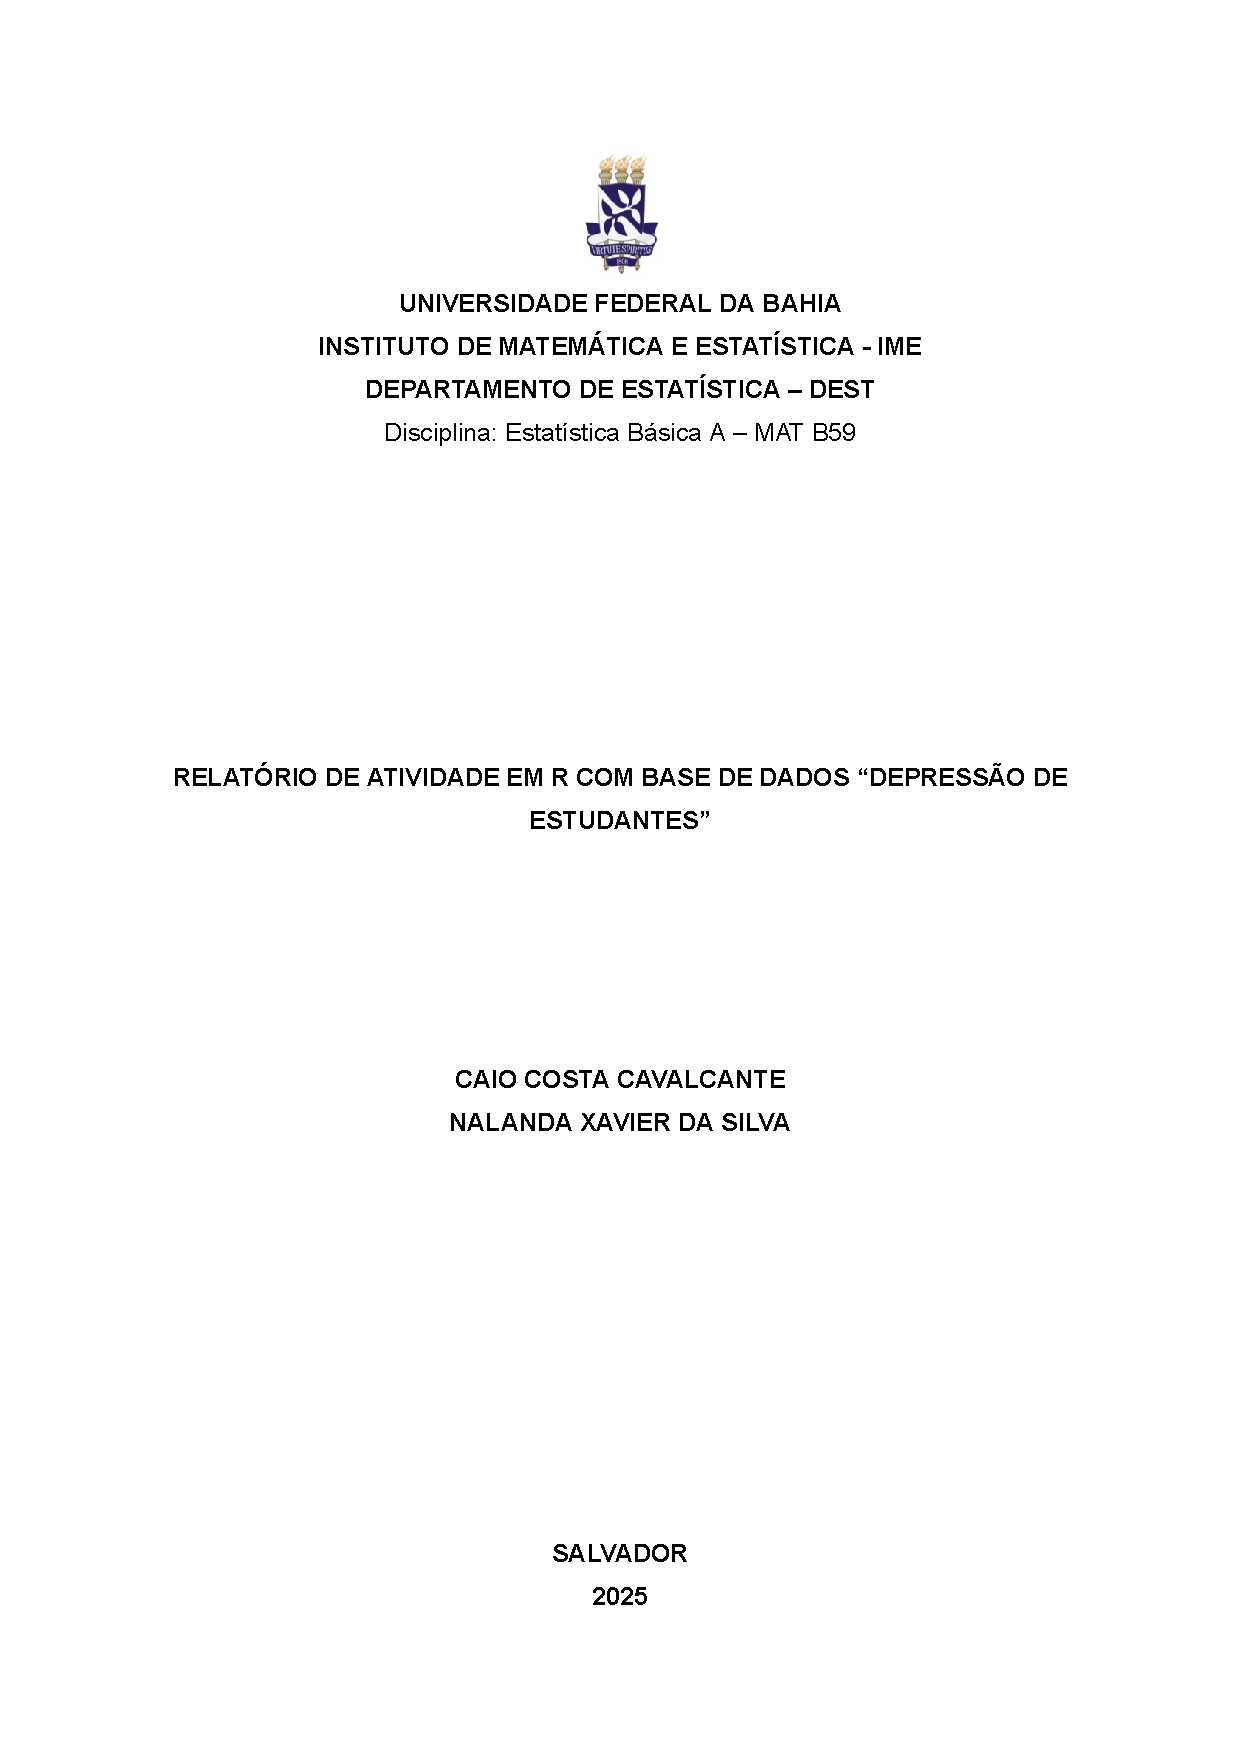
\includepdf[pages=-]{Relatório científico - Nalanda Xavier da Silva e Caio Costa Cavalcante.pdf}

\section{Apêndice -- Código R Completo}\label{apendice}

\begin{Shaded}
\begin{Highlighting}[]
\CommentTok{\# ==== Início: preprocessamento.R ====}
\CommentTok{\# instalando os pacotes}
\FunctionTok{install.packages}\NormalTok{(}\StringTok{"readr"}\NormalTok{)}
\FunctionTok{install.packages}\NormalTok{(}\StringTok{"janitor"}\NormalTok{)}
\FunctionTok{install.packages}\NormalTok{(}\StringTok{"flextable"}\NormalTok{)}
\FunctionTok{install.packages}\NormalTok{(}\StringTok{"tidyverse"}\NormalTok{)}

\CommentTok{\# carregando os pacotes}
\FunctionTok{library}\NormalTok{(dplyr) }
\FunctionTok{library}\NormalTok{(janitor)}
\FunctionTok{library}\NormalTok{(flextable)  }
\FunctionTok{library}\NormalTok{(tidyverse)}
\FunctionTok{library}\NormalTok{(ggplot2) }
\CommentTok{\# ==== Fim do Preprocessamento ====}

\CommentTok{\# Função utilitária para formatar percentuais com duas casas decimais e vírgula}
\NormalTok{format\_pct }\OtherTok{\textless{}{-}} \ControlFlowTok{function}\NormalTok{(x) \{}
  \FunctionTok{format}\NormalTok{(}\FunctionTok{round}\NormalTok{(x, }\DecValTok{2}\NormalTok{), }\AttributeTok{nsmall =} \DecValTok{2}\NormalTok{, }\AttributeTok{decimal.mark =} \StringTok{","}\NormalTok{)}
\NormalTok{\}}


\CommentTok{\#carregando os dados}
\NormalTok{base }\OtherTok{\textless{}{-}} \FunctionTok{read\_csv}\NormalTok{(}\StringTok{"estudantes\_depressao.csv"}\NormalTok{)}


\CommentTok{\#visualizando os dados}
\FunctionTok{head}\NormalTok{(base)}


\CommentTok{\#Pensamento Suicidas}

\CommentTok{\# Salvando a variável com os dados}
\NormalTok{pensamentos\_suicidas }\OtherTok{\textless{}{-}}\NormalTok{ base}\SpecialCharTok{$}\NormalTok{voce\_ja\_teve\_pensamentos\_suicidas}

\CommentTok{\# Frequência absoluta e relativa}
\NormalTok{pensamentos\_suicidas\_freq }\OtherTok{\textless{}{-}} \FunctionTok{table}\NormalTok{(pensamentos\_suicidas)}
\NormalTok{pensamentos\_suicidas\_rel }\OtherTok{\textless{}{-}} \FunctionTok{prop.table}\NormalTok{(pensamentos\_suicidas\_freq)}

\CommentTok{\# Criando dataframe}
\NormalTok{pensamentos\_suicidas\_df }\OtherTok{\textless{}{-}} \FunctionTok{data.frame}\NormalTok{(}
  \AttributeTok{Pensamentos\_Suicidas =} \FunctionTok{names}\NormalTok{(pensamentos\_suicidas\_freq),}
  \AttributeTok{Frequencia =} \FunctionTok{as.numeric}\NormalTok{(pensamentos\_suicidas\_freq),}
  \AttributeTok{Percentual =} \FunctionTok{as.numeric}\NormalTok{(pensamentos\_suicidas\_rel)}\SpecialCharTok{*}\DecValTok{100}
\NormalTok{) }\SpecialCharTok{\%\textgreater{}\%}
  \FunctionTok{mutate}\NormalTok{(}\AttributeTok{Percentual =} \FunctionTok{format\_pct}\NormalTok{(Percentual))}

\CommentTok{\# Tabela flextable}
\NormalTok{pensamentos\_suicidas\_ft }\OtherTok{\textless{}{-}} \FunctionTok{flextable}\NormalTok{(pensamentos\_suicidas\_df) }\SpecialCharTok{\%\textgreater{}\%}
  \FunctionTok{set\_caption}\NormalTok{(}\StringTok{"Tabela 1 – Percentual de Pensamentos Suicidas Estudantes na Índia"}\NormalTok{) }\SpecialCharTok{\%\textgreater{}\%}
  \FunctionTok{set\_header\_labels}\NormalTok{(}\AttributeTok{Pensamentos\_Suicidas=}\StringTok{"Pensamentos Suicidas"}\NormalTok{, }\AttributeTok{Frequencia=}\StringTok{"Quantidade"}\NormalTok{, }\AttributeTok{Percentual=}\StringTok{"Percentual (\%)"}\NormalTok{) }\SpecialCharTok{\%\textgreater{}\%}
  \FunctionTok{theme\_vanilla}\NormalTok{() }\SpecialCharTok{\%\textgreater{}\%}
  \FunctionTok{set\_table\_properties}\NormalTok{(}\AttributeTok{width=}\FloatTok{0.5}\NormalTok{, }\AttributeTok{layout=}\StringTok{"autofit"}\NormalTok{) }\SpecialCharTok{\%\textgreater{}\%}
  \FunctionTok{add\_footer\_lines}\NormalTok{(}\FunctionTok{c}\NormalTok{(}\StringTok{"Fonte: Depression Student Dataset (Primeiro semestre de 2023)"}\NormalTok{, }\FunctionTok{paste}\NormalTok{(}\StringTok{"Data da análise:"}\NormalTok{, }\FunctionTok{format}\NormalTok{(}\FunctionTok{Sys.Date}\NormalTok{(), }\StringTok{"\%d/\%m/\%Y"}\NormalTok{))))}

\CommentTok{\# Exibir tabela}
\FunctionTok{print}\NormalTok{(pensamentos\_suicidas\_ft)}

\CommentTok{\# Tabela 1 feita no código acima}

\CommentTok{\# Gráfico de pizza}

\NormalTok{pensamentos\_suicidas\_df }\OtherTok{\textless{}{-}}\NormalTok{ pensamentos\_suicidas\_df }\SpecialCharTok{\%\textgreater{}\%} \FunctionTok{mutate}\NormalTok{(}\AttributeTok{PercentualNum =} \FunctionTok{as.numeric}\NormalTok{(}\FunctionTok{gsub}\NormalTok{(}\StringTok{","}\NormalTok{,}\StringTok{"."}\NormalTok{,Percentual)))}

\FunctionTok{ggplot}\NormalTok{(pensamentos\_suicidas\_df, }\FunctionTok{aes}\NormalTok{(}\AttributeTok{x=}\StringTok{""}\NormalTok{, }\AttributeTok{y=}\NormalTok{PercentualNum, }\AttributeTok{fill=}\NormalTok{Pensamentos\_Suicidas)) }\SpecialCharTok{+}
  \FunctionTok{geom\_bar}\NormalTok{(}\AttributeTok{stat=}\StringTok{"identity"}\NormalTok{, }\AttributeTok{width=}\DecValTok{1}\NormalTok{) }\SpecialCharTok{+}
  \FunctionTok{coord\_polar}\NormalTok{(}\StringTok{"y"}\NormalTok{) }\SpecialCharTok{+}
  \FunctionTok{geom\_label}\NormalTok{(}\FunctionTok{aes}\NormalTok{(}\AttributeTok{label=}\FunctionTok{paste0}\NormalTok{(Pensamentos\_Suicidas,}\StringTok{"}\SpecialCharTok{\textbackslash{}n}\StringTok{"}\NormalTok{,Percentual,}\StringTok{"\%"}\NormalTok{)), }\AttributeTok{position=}\FunctionTok{position\_stack}\NormalTok{(}\AttributeTok{vjust=}\FloatTok{0.5}\NormalTok{), }\AttributeTok{size=}\DecValTok{4}\NormalTok{) }\SpecialCharTok{+}
  \FunctionTok{labs}\NormalTok{(}\AttributeTok{title=}\StringTok{"Gráfico 1 – Distribuição Percentual de Pensamentos Suicidas na Índia"}\NormalTok{, }\AttributeTok{fill=}\StringTok{"Pensamentos Suicidas"}\NormalTok{, }\AttributeTok{caption=}\FunctionTok{paste}\NormalTok{(}\StringTok{"Fonte: Depression Student Dataset (2023)}\SpecialCharTok{\textbackslash{}n}\StringTok{Data da análise:"}\NormalTok{, }\FunctionTok{format}\NormalTok{(}\FunctionTok{Sys.Date}\NormalTok{(), }\StringTok{"\%d/\%m/\%Y"}\NormalTok{))) }\SpecialCharTok{+}
  \FunctionTok{theme\_void}\NormalTok{() }\SpecialCharTok{+}
  \FunctionTok{theme}\NormalTok{(}\AttributeTok{legend.position=}\StringTok{"right"}\NormalTok{, }\AttributeTok{plot.caption=}\FunctionTok{element\_text}\NormalTok{(}\AttributeTok{hjust=}\FloatTok{0.5}\NormalTok{, }\AttributeTok{face=}\StringTok{"italic"}\NormalTok{, }\AttributeTok{size=}\DecValTok{8}\NormalTok{))}
\CommentTok{\# ==== Fim de Pensamento suicida ====}

\CommentTok{\# Pressão Acadêmica}

\CommentTok{\# Salvando pressão academica em uma variável}
\NormalTok{nivel\_pressao\_academica }\OtherTok{\textless{}{-}}\NormalTok{ base}\SpecialCharTok{$}\NormalTok{nivel\_de\_pressao\_academica}

\CommentTok{\# Frequência absoluta e relativa}
\NormalTok{nivel\_pressao\_academica\_freq }\OtherTok{\textless{}{-}} \FunctionTok{table}\NormalTok{(nivel\_pressao\_academica)}
\NormalTok{nivel\_pressao\_academica\_rel }\OtherTok{\textless{}{-}} \FunctionTok{prop.table}\NormalTok{(nivel\_pressao\_academica\_freq)}

\NormalTok{nivel\_pressao\_academica\_df }\OtherTok{\textless{}{-}} \FunctionTok{data.frame}\NormalTok{(}
  \AttributeTok{Nivel\_Pressao\_Academica =} \FunctionTok{names}\NormalTok{(nivel\_pressao\_academica\_freq),}
  \AttributeTok{Frequencia =} \FunctionTok{as.numeric}\NormalTok{(nivel\_pressao\_academica\_freq),}
  \AttributeTok{Percentual =} \FunctionTok{as.numeric}\NormalTok{(nivel\_pressao\_academica\_rel)}\SpecialCharTok{*}\DecValTok{100}
\NormalTok{) }\SpecialCharTok{\%\textgreater{}\%}
  \FunctionTok{mutate}\NormalTok{(}\AttributeTok{Percentual =} \FunctionTok{format}\NormalTok{(}\FunctionTok{round}\NormalTok{(Percentual,}\DecValTok{2}\NormalTok{), }\AttributeTok{nsmall =} \DecValTok{2}\NormalTok{, }\AttributeTok{decimal.mark=}\StringTok{","}\NormalTok{))}

\NormalTok{nivel\_pressao\_academica\_ft }\OtherTok{\textless{}{-}} \FunctionTok{flextable}\NormalTok{(nivel\_pressao\_academica\_df) }\SpecialCharTok{\%\textgreater{}\%}
  \FunctionTok{set\_caption}\NormalTok{(}\StringTok{"Tabela 2 – Frequência e Percentual de Nível de Pressão Acadêmica"}\NormalTok{) }\SpecialCharTok{\%\textgreater{}\%}
  \FunctionTok{set\_header\_labels}\NormalTok{(}\AttributeTok{Nivel\_Pressao\_Academica=}\StringTok{"Nível de Pressão Acadêmica"}\NormalTok{, }\AttributeTok{Frequencia=}\StringTok{"Quantidade"}\NormalTok{, }\AttributeTok{Percentual=}\StringTok{"Percentual (\%)"}\NormalTok{) }\SpecialCharTok{\%\textgreater{}\%}
  \FunctionTok{theme\_vanilla}\NormalTok{() }\SpecialCharTok{\%\textgreater{}\%}
  \FunctionTok{set\_table\_properties}\NormalTok{(}\AttributeTok{width=}\FloatTok{0.5}\NormalTok{, }\AttributeTok{layout=}\StringTok{"autofit"}\NormalTok{) }\SpecialCharTok{\%\textgreater{}\%}
  \FunctionTok{add\_footer\_lines}\NormalTok{(}\FunctionTok{c}\NormalTok{(}\StringTok{"Fonte: Depression Student Dataset (2023)"}\NormalTok{, }\FunctionTok{paste}\NormalTok{(}\StringTok{"Data da análise:"}\NormalTok{, }\FunctionTok{format}\NormalTok{(}\FunctionTok{Sys.Date}\NormalTok{(), }\StringTok{"\%d/\%m/\%Y"}\NormalTok{))))}

\FunctionTok{print}\NormalTok{(nivel\_pressao\_academica\_ft)}

\CommentTok{\# Resumo estatístico}
\CommentTok{\# Resumo estatístico da variável}
\NormalTok{resumo\_pressao\_academica }\OtherTok{\textless{}{-}} \FunctionTok{summary}\NormalTok{(nivel\_pressao\_academica)}

\CommentTok{\# Transformar em data.frame}
\NormalTok{resumo\_pressao\_academica\_df }\OtherTok{\textless{}{-}} \FunctionTok{data.frame}\NormalTok{(}
  \AttributeTok{Estatistica =} \FunctionTok{names}\NormalTok{(resumo\_pressao\_academica),}
  \AttributeTok{Valor =} \FunctionTok{as.numeric}\NormalTok{(resumo\_pressao\_academica)}
\NormalTok{)}

\CommentTok{\# Renomear para nomes mais amigáveis}
\NormalTok{resumo\_pressao\_academica\_df}\SpecialCharTok{$}\NormalTok{Estatistica }\OtherTok{\textless{}{-}} \FunctionTok{recode}\NormalTok{(resumo\_pressao\_academica\_df}\SpecialCharTok{$}\NormalTok{Estatistica,}
                                                  \StringTok{"Min."}     \OtherTok{=} \StringTok{"Pressão Mínima"}\NormalTok{,  }
                                                  \StringTok{"1st Qu."}  \OtherTok{=} \StringTok{"2 ou menor"}\NormalTok{,}
                                                  \StringTok{"Median"}   \OtherTok{=} \StringTok{"Pressão Moderada"}\NormalTok{,}
                                                  \StringTok{"Mean"}     \OtherTok{=} \StringTok{"Média"}\NormalTok{,}
                                                  \StringTok{"3rd Qu."}  \OtherTok{=} \StringTok{"4 ou mais (Alto)"}\NormalTok{,}
                                                  \StringTok{"Max."}     \OtherTok{=} \StringTok{"Muita Pressão"}\NormalTok{)}

\CommentTok{\# Criar a flextable com título e fonte corrigindo o erro de format()}
\NormalTok{resumo\_pressao\_academica\_ft }\OtherTok{\textless{}{-}} \FunctionTok{flextable}\NormalTok{(resumo\_pressao\_academica\_df) }\SpecialCharTok{\%\textgreater{}\%}
  \FunctionTok{set\_header\_labels}\NormalTok{(}\AttributeTok{Estatistica =} \StringTok{"Estatística"}\NormalTok{, }\AttributeTok{Valor =} \StringTok{"Valor"}\NormalTok{) }\SpecialCharTok{\%\textgreater{}\%}
  \FunctionTok{theme\_vanilla}\NormalTok{() }\SpecialCharTok{\%\textgreater{}\%}
  \FunctionTok{set\_caption}\NormalTok{(}\StringTok{"Tabela 3 – Níveis de Pressão Acadêmica na Índia"}\NormalTok{) }\SpecialCharTok{\%\textgreater{}\%}
  \FunctionTok{add\_footer\_lines}\NormalTok{(}\AttributeTok{values =} \FunctionTok{c}\NormalTok{(}
    \StringTok{"Fonte: Depression Student Dataset (2023)"}\NormalTok{,}
    \FunctionTok{paste}\NormalTok{(}\StringTok{"Data da análise:"}\NormalTok{, }\FunctionTok{format}\NormalTok{(}\FunctionTok{Sys.Date}\NormalTok{(), }\StringTok{"\%d/\%m/\%Y"}\NormalTok{))}
\NormalTok{  )) }\SpecialCharTok{\%\textgreater{}\%}
  \FunctionTok{set\_table\_properties}\NormalTok{(}\AttributeTok{width =} \FloatTok{0.5}\NormalTok{, }\AttributeTok{layout =} \StringTok{"autofit"}\NormalTok{)}

\CommentTok{\# Exibir a tabela}
\NormalTok{resumo\_pressao\_academica\_ft}


\CommentTok{\# Gráfico de barras}
\FunctionTok{ggplot}\NormalTok{(nivel\_pressao\_academica\_df, }\FunctionTok{aes}\NormalTok{(}\AttributeTok{x =}\NormalTok{ Nivel\_Pressao\_Academica, }\AttributeTok{y =}\NormalTok{ Percentual, }\AttributeTok{fill =}\NormalTok{ Nivel\_Pressao\_Academica)) }\SpecialCharTok{+}
  \FunctionTok{geom\_bar}\NormalTok{(}\AttributeTok{stat =} \StringTok{"identity"}\NormalTok{) }\SpecialCharTok{+}
  \FunctionTok{geom\_text}\NormalTok{(}\FunctionTok{aes}\NormalTok{(}\AttributeTok{label =} \FunctionTok{paste0}\NormalTok{(Percentual, }\StringTok{"\%"}\NormalTok{)), }\AttributeTok{vjust =} \SpecialCharTok{{-}}\FloatTok{0.5}\NormalTok{, }\AttributeTok{size =} \DecValTok{4}\NormalTok{) }\SpecialCharTok{+}
  \FunctionTok{labs}\NormalTok{(}
    \AttributeTok{title =} \StringTok{"Gráfico 2 – Nível de Pressão Acadêmica na Índia"}\NormalTok{,}
    \AttributeTok{x =} \StringTok{"Nível de Pressão Acadêmica"}\NormalTok{,}
    \AttributeTok{y =} \StringTok{"Percentual (\%)"}\NormalTok{,}
    \AttributeTok{fill =} \StringTok{"Nível de Pressão Acadêmica"}\NormalTok{,}
    \AttributeTok{caption =} \FunctionTok{paste}\NormalTok{(}\StringTok{"Fonte: Depression Student Dataset (2023)}\SpecialCharTok{\textbackslash{}n}\StringTok{Data da análise:"}\NormalTok{, }\FunctionTok{format}\NormalTok{(}\FunctionTok{Sys.Date}\NormalTok{(), }\StringTok{"\%d/\%m/\%Y"}\NormalTok{))}
\NormalTok{  ) }\SpecialCharTok{+}
  \FunctionTok{theme\_minimal}\NormalTok{() }\SpecialCharTok{+}
  \FunctionTok{theme}\NormalTok{(}
    \AttributeTok{legend.position =} \StringTok{"right"}\NormalTok{,}
    \AttributeTok{plot.title =} \FunctionTok{element\_text}\NormalTok{(}\AttributeTok{hjust =} \FloatTok{0.5}\NormalTok{)}
\NormalTok{  )}

\CommentTok{\# ==== Fim de Pressão academica ====}

\CommentTok{\# Duração do Sono}

\CommentTok{\# Salvando duração de sono em uma variável}
\NormalTok{duracao\_sono }\OtherTok{\textless{}{-}}\NormalTok{ base}\SpecialCharTok{$}\NormalTok{duracao\_do\_sono}

\CommentTok{\# Frequência absoluta e relativa}
\NormalTok{duracao\_sono\_freq }\OtherTok{\textless{}{-}} \FunctionTok{table}\NormalTok{(duracao\_sono)}
\NormalTok{duracao\_sono\_rel }\OtherTok{\textless{}{-}} \FunctionTok{prop.table}\NormalTok{(duracao\_sono\_freq)}

\NormalTok{duracao\_sono\_df }\OtherTok{\textless{}{-}} \FunctionTok{data.frame}\NormalTok{(}
  \AttributeTok{Duracao\_Sono =} \FunctionTok{names}\NormalTok{(duracao\_sono\_freq),}
  \AttributeTok{Frequencia =} \FunctionTok{as.numeric}\NormalTok{(duracao\_sono\_freq),}
  \AttributeTok{Percentual =} \FunctionTok{as.numeric}\NormalTok{(duracao\_sono\_rel)}\SpecialCharTok{*}\DecValTok{100}
\NormalTok{) }\SpecialCharTok{\%\textgreater{}\%}
  \FunctionTok{mutate}\NormalTok{(}\AttributeTok{Percentual =} \FunctionTok{format}\NormalTok{(}\FunctionTok{round}\NormalTok{(Percentual,}\DecValTok{2}\NormalTok{), }\AttributeTok{nsmall =} \DecValTok{2}\NormalTok{, }\AttributeTok{decimal.mark=}\StringTok{","}\NormalTok{))}

\NormalTok{duracao\_sono\_ft }\OtherTok{\textless{}{-}} \FunctionTok{flextable}\NormalTok{(duracao\_sono\_df) }\SpecialCharTok{\%\textgreater{}\%}
  \FunctionTok{set\_caption}\NormalTok{(}\StringTok{"Tabela 4 – Frequência e Percentual de Duração do Sono"}\NormalTok{) }\SpecialCharTok{\%\textgreater{}\%}
  \FunctionTok{set\_header\_labels}\NormalTok{(}\AttributeTok{Duracao\_Sono=}\StringTok{"Duração do Sono"}\NormalTok{, }\AttributeTok{Frequencia=}\StringTok{"Quantidade"}\NormalTok{, }\AttributeTok{Percentual=}\StringTok{"Percentual (\%)"}\NormalTok{) }\SpecialCharTok{\%\textgreater{}\%}
  \FunctionTok{theme\_vanilla}\NormalTok{() }\SpecialCharTok{\%\textgreater{}\%}
  \FunctionTok{set\_table\_properties}\NormalTok{(}\AttributeTok{width=}\FloatTok{0.5}\NormalTok{, }\AttributeTok{layout=}\StringTok{"autofit"}\NormalTok{) }\SpecialCharTok{\%\textgreater{}\%}
  \FunctionTok{add\_footer\_lines}\NormalTok{(}\FunctionTok{c}\NormalTok{(}\StringTok{"Fonte: Depression Student Dataset (2023)"}\NormalTok{, }\FunctionTok{paste}\NormalTok{(}\StringTok{"Data da análise:"}\NormalTok{, }\FunctionTok{format}\NormalTok{(}\FunctionTok{Sys.Date}\NormalTok{(), }\StringTok{"\%d/\%m/\%Y"}\NormalTok{))))}

\FunctionTok{print}\NormalTok{(duracao\_sono\_ft)}

\CommentTok{\# Gráfico de barras}
\FunctionTok{ggplot}\NormalTok{(duracao\_sono\_df, }\FunctionTok{aes}\NormalTok{(}\AttributeTok{x =}\NormalTok{ Duracao\_Sono, }\AttributeTok{y =}\NormalTok{ Percentual, }\AttributeTok{fill =}\NormalTok{ Duracao\_Sono)) }\SpecialCharTok{+}
  \FunctionTok{geom\_bar}\NormalTok{(}\AttributeTok{stat =} \StringTok{"identity"}\NormalTok{) }\SpecialCharTok{+}
  \FunctionTok{geom\_text}\NormalTok{(}\FunctionTok{aes}\NormalTok{(}\AttributeTok{label =} \FunctionTok{paste0}\NormalTok{(Percentual, }\StringTok{"\%"}\NormalTok{)), }\AttributeTok{vjust =} \SpecialCharTok{{-}}\FloatTok{0.5}\NormalTok{, }\AttributeTok{size =} \DecValTok{4}\NormalTok{) }\SpecialCharTok{+}
  \FunctionTok{labs}\NormalTok{(}
    \AttributeTok{title =} \StringTok{"Gráfico 3 – Duração do Sono na Índia"}\NormalTok{,}
    \AttributeTok{x =} \StringTok{"Duração do Sono"}\NormalTok{,}
    \AttributeTok{y =} \StringTok{"Percentual (\%)"}\NormalTok{,}
    \AttributeTok{fill =} \StringTok{"Duração do Sono"}\NormalTok{,}
    \AttributeTok{caption =} \FunctionTok{paste}\NormalTok{(}\StringTok{"Fonte: Depression Student Dataset (2023)}\SpecialCharTok{\textbackslash{}n}\StringTok{Data da análise:"}\NormalTok{, }\FunctionTok{format}\NormalTok{(}\FunctionTok{Sys.Date}\NormalTok{(), }\StringTok{"\%d/\%m/\%Y"}\NormalTok{))}
\NormalTok{  ) }\SpecialCharTok{+}
  \FunctionTok{theme\_minimal}\NormalTok{() }\SpecialCharTok{+}
  \FunctionTok{theme}\NormalTok{(}
    \AttributeTok{legend.position =} \StringTok{"right"}\NormalTok{,}
    \AttributeTok{plot.title =} \FunctionTok{element\_text}\NormalTok{(}\AttributeTok{hjust =} \FloatTok{0.5}\NormalTok{)}
\NormalTok{  )}
\CommentTok{\# ==== Fim de Duração Sono ====}

\CommentTok{\# Gênero}
\CommentTok{\# Salvando gênero em uma variável}
\NormalTok{genero }\OtherTok{\textless{}{-}}\NormalTok{ base}\SpecialCharTok{$}\NormalTok{genero}
\CommentTok{\# Frequência absoluta e relativa}

\NormalTok{genero\_freq }\OtherTok{\textless{}{-}} \FunctionTok{table}\NormalTok{(genero)}
\NormalTok{genero\_rel }\OtherTok{\textless{}{-}} \FunctionTok{prop.table}\NormalTok{(genero\_freq)}

\CommentTok{\# Criando dataframe com duas casas decimais e vírgula no percentual}
\NormalTok{genero\_df }\OtherTok{\textless{}{-}} \FunctionTok{data.frame}\NormalTok{(}
  \AttributeTok{Genero =} \FunctionTok{names}\NormalTok{(genero\_freq),}
  \AttributeTok{Frequencia =} \FunctionTok{as.numeric}\NormalTok{(genero\_freq),}
  \AttributeTok{Percentual =} \FunctionTok{as.numeric}\NormalTok{(genero\_rel)}\SpecialCharTok{*}\DecValTok{100}
\NormalTok{) }\SpecialCharTok{\%\textgreater{}\%}
  \FunctionTok{mutate}\NormalTok{(}\AttributeTok{Percentual =} \FunctionTok{format}\NormalTok{(}\FunctionTok{round}\NormalTok{(Percentual,}\DecValTok{2}\NormalTok{), }\AttributeTok{nsmall =} \DecValTok{2}\NormalTok{, }\AttributeTok{decimal.mark=}\StringTok{","}\NormalTok{))}

\CommentTok{\# Tabela flextable}
\NormalTok{genero\_ft }\OtherTok{\textless{}{-}} \FunctionTok{flextable}\NormalTok{(genero\_df) }\SpecialCharTok{\%\textgreater{}\%}
  \FunctionTok{set\_caption}\NormalTok{(}\StringTok{"Tabela 5 – Frequência e Percentual de Gênero"}\NormalTok{) }\SpecialCharTok{\%\textgreater{}\%}
  \FunctionTok{set\_header\_labels}\NormalTok{(}\AttributeTok{Genero=}\StringTok{"Gênero"}\NormalTok{, }\AttributeTok{Frequencia=}\StringTok{"Quantidade"}\NormalTok{, }\AttributeTok{Percentual=}\StringTok{"Percentual (\%)"}\NormalTok{) }\SpecialCharTok{\%\textgreater{}\%}
  \FunctionTok{theme\_vanilla}\NormalTok{() }\SpecialCharTok{\%\textgreater{}\%}
  \FunctionTok{set\_table\_properties}\NormalTok{(}\AttributeTok{width=}\FloatTok{0.5}\NormalTok{, }\AttributeTok{layout=}\StringTok{"autofit"}\NormalTok{) }\SpecialCharTok{\%\textgreater{}\%}
  \FunctionTok{add\_footer\_lines}\NormalTok{(}\FunctionTok{c}\NormalTok{(}\StringTok{"Fonte: Depression Student Dataset (2023)"}\NormalTok{, }\FunctionTok{paste}\NormalTok{(}\StringTok{"Data da análise:"}\NormalTok{, }\FunctionTok{format}\NormalTok{(}\FunctionTok{Sys.Date}\NormalTok{(), }\StringTok{"\%d/\%m/\%Y"}\NormalTok{))))}

\CommentTok{\# Exibir tabela}
\FunctionTok{print}\NormalTok{(genero\_ft)}
\CommentTok{\# Gráfico de barras}
\FunctionTok{ggplot}\NormalTok{(genero\_df, }\FunctionTok{aes}\NormalTok{(}\AttributeTok{x =}\NormalTok{ Genero, }\AttributeTok{y =}\NormalTok{ Percentual, }\AttributeTok{fill =}\NormalTok{ Genero)) }\SpecialCharTok{+}
  \FunctionTok{geom\_bar}\NormalTok{(}\AttributeTok{stat =} \StringTok{"identity"}\NormalTok{) }\SpecialCharTok{+}
  \FunctionTok{geom\_text}\NormalTok{(}\FunctionTok{aes}\NormalTok{(}\AttributeTok{label =} \FunctionTok{paste0}\NormalTok{(Percentual, }\StringTok{"\%"}\NormalTok{)), }\AttributeTok{vjust =} \SpecialCharTok{{-}}\FloatTok{0.5}\NormalTok{, }\AttributeTok{size =} \DecValTok{4}\NormalTok{) }\SpecialCharTok{+}
  \FunctionTok{labs}\NormalTok{(}
    \AttributeTok{title =} \StringTok{"Gráfico 4 – Distribuição de Gênero dos Estudantes da Índia"}\NormalTok{,}
    \AttributeTok{x =} \StringTok{"Gênero"}\NormalTok{,}
    \AttributeTok{y =} \StringTok{"Percentual (\%)"}\NormalTok{,}
    \AttributeTok{fill =} \StringTok{"Gênero"}\NormalTok{,}
    \AttributeTok{caption =} \FunctionTok{paste}\NormalTok{(}\StringTok{"Fonte: Depression Student Dataset (2023)}\SpecialCharTok{\textbackslash{}n}\StringTok{Data da análise:"}\NormalTok{, }\FunctionTok{format}\NormalTok{(}\FunctionTok{Sys.Date}\NormalTok{(), }\StringTok{"\%d/\%m/\%Y"}\NormalTok{))}
\NormalTok{  ) }\SpecialCharTok{+}
  \FunctionTok{theme\_minimal}\NormalTok{() }\SpecialCharTok{+}
  \FunctionTok{theme}\NormalTok{(}
    \AttributeTok{legend.position =} \StringTok{"right"}\NormalTok{,}
    \AttributeTok{plot.title =} \FunctionTok{element\_text}\NormalTok{(}\AttributeTok{hjust =} \FloatTok{0.5}\NormalTok{)}
\NormalTok{  )}

\CommentTok{\# ==== Fim de Gênero ====}

\CommentTok{\# Idade}
\CommentTok{\# Salvando idade em uma variável}
\NormalTok{idade }\OtherTok{\textless{}{-}}\NormalTok{ base}\SpecialCharTok{$}\NormalTok{idade}

\CommentTok{\# Análise estatística com valores arredondados e nomes acessíveis}
\NormalTok{idade\_stats }\OtherTok{\textless{}{-}} \FunctionTok{data.frame}\NormalTok{(}
  \AttributeTok{Estatistica =} \FunctionTok{c}\NormalTok{(}\StringTok{"Idade Média"}\NormalTok{, }\StringTok{"Mediana da Idade"}\NormalTok{, }\StringTok{"Variação da Idade"}\NormalTok{, }\StringTok{"Idade Mínima"}\NormalTok{, }\StringTok{"Idade Máxima"}\NormalTok{),}
  \AttributeTok{Valor =} \FunctionTok{c}\NormalTok{(}
    \FunctionTok{mean}\NormalTok{(idade, }\AttributeTok{na.rm =} \ConstantTok{TRUE}\NormalTok{),}
    \FunctionTok{median}\NormalTok{(idade, }\AttributeTok{na.rm =} \ConstantTok{TRUE}\NormalTok{),}
    \FunctionTok{sd}\NormalTok{(idade, }\AttributeTok{na.rm =} \ConstantTok{TRUE}\NormalTok{),}
    \FunctionTok{min}\NormalTok{(idade, }\AttributeTok{na.rm =} \ConstantTok{TRUE}\NormalTok{),}
    \FunctionTok{max}\NormalTok{(idade, }\AttributeTok{na.rm =} \ConstantTok{TRUE}\NormalTok{)}
\NormalTok{  )}
\NormalTok{) }\SpecialCharTok{\%\textgreater{}\%}
  \FunctionTok{mutate}\NormalTok{(}\AttributeTok{Valor =} \FunctionTok{format}\NormalTok{(}\FunctionTok{round}\NormalTok{(Valor, }\DecValTok{2}\NormalTok{), }\AttributeTok{nsmall =} \DecValTok{2}\NormalTok{, }\AttributeTok{decimal.mark =} \StringTok{","}\NormalTok{))  }\CommentTok{\# Duas casas decimais, vírgula como separador}

\CommentTok{\# Criando a flextable}
\NormalTok{idade\_stats\_ft }\OtherTok{\textless{}{-}} \FunctionTok{flextable}\NormalTok{(idade\_stats) }\SpecialCharTok{\%\textgreater{}\%}
  \FunctionTok{set\_caption}\NormalTok{(}\StringTok{"Tabela 6 – Estatísticas Descritivas da Idade dos Estudantes"}\NormalTok{) }\SpecialCharTok{\%\textgreater{}\%}
  \FunctionTok{set\_header\_labels}\NormalTok{(}\AttributeTok{Estatistica =} \StringTok{"Estatística"}\NormalTok{, }\AttributeTok{Valor =} \StringTok{"Valor (anos)"}\NormalTok{) }\SpecialCharTok{\%\textgreater{}\%}
  \FunctionTok{theme\_vanilla}\NormalTok{() }\SpecialCharTok{\%\textgreater{}\%}
  \FunctionTok{set\_table\_properties}\NormalTok{(}\AttributeTok{width =} \FloatTok{0.5}\NormalTok{, }\AttributeTok{layout =} \StringTok{"autofit"}\NormalTok{) }\SpecialCharTok{\%\textgreater{}\%}
  \FunctionTok{add\_footer\_lines}\NormalTok{(}\FunctionTok{c}\NormalTok{(}
    \StringTok{"Fonte: Depression Student Dataset (2023)"}\NormalTok{, }
    \FunctionTok{paste}\NormalTok{(}\StringTok{"Data da análise:"}\NormalTok{, }\FunctionTok{format}\NormalTok{(}\FunctionTok{Sys.Date}\NormalTok{(), }\StringTok{"\%d/\%m/\%Y"}\NormalTok{))}
\NormalTok{  ))}

\CommentTok{\# Exibir tabela}
\FunctionTok{print}\NormalTok{(idade\_stats\_ft)}

\CommentTok{\# Histograma de idade}
\FunctionTok{ggplot}\NormalTok{(base, }\FunctionTok{aes}\NormalTok{(}\AttributeTok{x =}\NormalTok{ idade)) }\SpecialCharTok{+}
  \FunctionTok{geom\_histogram}\NormalTok{(}\AttributeTok{binwidth =} \DecValTok{1}\NormalTok{, }\AttributeTok{fill =} \StringTok{"\#69b3a2"}\NormalTok{, }\AttributeTok{color =} \StringTok{"black"}\NormalTok{, }\AttributeTok{alpha =} \FloatTok{0.7}\NormalTok{) }\SpecialCharTok{+}
  \FunctionTok{labs}\NormalTok{(}
    \AttributeTok{title =} \StringTok{"Gráfico 5 – Histograma da Idade dos Estudantes da Índia"}\NormalTok{,}
    \AttributeTok{x =} \StringTok{"Idade (anos)"}\NormalTok{,}
    \AttributeTok{y =} \StringTok{"Frequência"}\NormalTok{,}
    \AttributeTok{caption =} \FunctionTok{paste}\NormalTok{(}\StringTok{"Fonte: Depression Student Dataset (2023)}\SpecialCharTok{\textbackslash{}n}\StringTok{Data da análise:"}\NormalTok{, }\FunctionTok{format}\NormalTok{(}\FunctionTok{Sys.Date}\NormalTok{(), }\StringTok{"\%d/\%m/\%Y"}\NormalTok{))}
\NormalTok{  ) }\SpecialCharTok{+}
  \FunctionTok{theme\_minimal}\NormalTok{() }\SpecialCharTok{+}
  \FunctionTok{theme}\NormalTok{(}\AttributeTok{plot.title =} \FunctionTok{element\_text}\NormalTok{(}\AttributeTok{hjust =} \FloatTok{0.5}\NormalTok{))}

\CommentTok{\# Gráfico de densidade de idade}
\FunctionTok{ggplot}\NormalTok{(base, }\FunctionTok{aes}\NormalTok{(}\AttributeTok{x =}\NormalTok{ idade)) }\SpecialCharTok{+}
  \FunctionTok{geom\_density}\NormalTok{(}\AttributeTok{fill =} \StringTok{"\#69b3a2"}\NormalTok{, }\AttributeTok{alpha =} \FloatTok{0.7}\NormalTok{) }\SpecialCharTok{+}
  \FunctionTok{labs}\NormalTok{(}
    \AttributeTok{title =} \StringTok{"Gráfico 6 – Densidade da Idade dos Estudantes da Índia"}\NormalTok{,}
    \AttributeTok{x =} \StringTok{"Idade (anos)"}\NormalTok{,}
    \AttributeTok{y =} \StringTok{"Densidade"}\NormalTok{,}
    \AttributeTok{caption =} \FunctionTok{paste}\NormalTok{(}\StringTok{"Fonte: Depression Student Dataset (2023)}\SpecialCharTok{\textbackslash{}n}\StringTok{Data da análise:"}\NormalTok{, }\FunctionTok{format}\NormalTok{(}\FunctionTok{Sys.Date}\NormalTok{(), }\StringTok{"\%d/\%m/\%Y"}\NormalTok{))}
\NormalTok{  ) }\SpecialCharTok{+}
  \FunctionTok{theme\_minimal}\NormalTok{() }\SpecialCharTok{+}
  \FunctionTok{theme}\NormalTok{(}\AttributeTok{plot.title =} \FunctionTok{element\_text}\NormalTok{(}\AttributeTok{hjust =} \FloatTok{0.5}\NormalTok{))}

\CommentTok{\# Gráfico violino}
\FunctionTok{ggplot}\NormalTok{(base, }\FunctionTok{aes}\NormalTok{(}\AttributeTok{x =} \StringTok{""}\NormalTok{, }\AttributeTok{y =}\NormalTok{ idade)) }\SpecialCharTok{+}
  \FunctionTok{geom\_violin}\NormalTok{(}\AttributeTok{fill =} \StringTok{"\#69b3a2"}\NormalTok{, }\AttributeTok{alpha =} \FloatTok{0.7}\NormalTok{) }\SpecialCharTok{+}
  \FunctionTok{labs}\NormalTok{(}
    \AttributeTok{title =} \StringTok{"Gráfico 7 – Gráfico Violino da Idade dos Estudantes da Índia"}\NormalTok{,}
    \AttributeTok{x =} \StringTok{""}\NormalTok{,}
    \AttributeTok{y =} \StringTok{"Idade (anos)"}\NormalTok{,}
    \AttributeTok{caption =} \FunctionTok{paste}\NormalTok{(}\StringTok{"Fonte: Depression Student Dataset (2023)}\SpecialCharTok{\textbackslash{}n}\StringTok{Data da análise:"}\NormalTok{, }\FunctionTok{format}\NormalTok{(}\FunctionTok{Sys.Date}\NormalTok{(), }\StringTok{"\%d/\%m/\%Y"}\NormalTok{))}
\NormalTok{  ) }\SpecialCharTok{+}
  \FunctionTok{theme\_minimal}\NormalTok{() }\SpecialCharTok{+}
  \FunctionTok{theme}\NormalTok{(}\AttributeTok{axis.title.x =} \FunctionTok{element\_blank}\NormalTok{(), }\AttributeTok{plot.title =} \FunctionTok{element\_text}\NormalTok{(}\AttributeTok{hjust =} \FloatTok{0.5}\NormalTok{))}
\CommentTok{\# ==== Fim de Idade ====}




\CommentTok{\# Análise de Gênero e Pensamentos Suicidas}
\CommentTok{\# Criando tabela cruzada}
\NormalTok{tabela\_cruzada }\OtherTok{\textless{}{-}} \FunctionTok{table}\NormalTok{(base}\SpecialCharTok{$}\NormalTok{genero, base}\SpecialCharTok{$}\NormalTok{voce\_ja\_teve\_pensamentos\_suicidas)}
\CommentTok{\# Convertendo para data.frame e calculando percentuais}
\NormalTok{tabela\_cruzada\_df }\OtherTok{\textless{}{-}} \FunctionTok{as.data.frame}\NormalTok{(tabela\_cruzada) }\SpecialCharTok{\%\textgreater{}\%}
  \FunctionTok{mutate}\NormalTok{(}\AttributeTok{Percentual =} \FunctionTok{format\_pct}\NormalTok{(Freq }\SpecialCharTok{/} \FunctionTok{sum}\NormalTok{(Freq) }\SpecialCharTok{*} \DecValTok{100}\NormalTok{))}
\CommentTok{\# Renomeando colunas}
\FunctionTok{colnames}\NormalTok{(tabela\_cruzada\_df) }\OtherTok{\textless{}{-}} \FunctionTok{c}\NormalTok{(}\StringTok{"Gênero"}\NormalTok{, }\StringTok{"Pensamentos\_Suicidas"}\NormalTok{, }\StringTok{"Frequencia"}\NormalTok{, }\StringTok{"Percentual"}\NormalTok{)}
\CommentTok{\# Criando flextable}
\NormalTok{tabela\_cruzada\_ft }\OtherTok{\textless{}{-}} \FunctionTok{flextable}\NormalTok{(tabela\_cruzada\_df) }\SpecialCharTok{\%\textgreater{}\%}
  \FunctionTok{set\_caption}\NormalTok{(}\StringTok{"Tabela 7 – Relação entre Gênero e Pensamentos Suicidas"}\NormalTok{) }\SpecialCharTok{\%\textgreater{}\%}
  \FunctionTok{set\_header\_labels}\NormalTok{(Gênero }\OtherTok{=} \StringTok{"Gênero"}\NormalTok{, }\AttributeTok{Pensamentos\_Suicidas =} \StringTok{"Pensamentos Suicidas"}\NormalTok{, }\AttributeTok{Frequencia =} \StringTok{"Frequência"}\NormalTok{, }\AttributeTok{Percentual =} \StringTok{"Percentual (\%)"}\NormalTok{) }\SpecialCharTok{\%\textgreater{}\%}
  \FunctionTok{theme\_vanilla}\NormalTok{() }\SpecialCharTok{\%\textgreater{}\%}
  \FunctionTok{set\_table\_properties}\NormalTok{(}\AttributeTok{width =} \FloatTok{0.5}\NormalTok{, }\AttributeTok{layout =} \StringTok{"autofit"}\NormalTok{) }\SpecialCharTok{\%\textgreater{}\%}
  \FunctionTok{add\_footer\_lines}\NormalTok{(}\FunctionTok{c}\NormalTok{(}
    \StringTok{"Fonte: Depression Student Dataset (2023)"}\NormalTok{,}
    \FunctionTok{paste}\NormalTok{(}\StringTok{"Data da análise:"}\NormalTok{, }\FunctionTok{format}\NormalTok{(}\FunctionTok{Sys.Date}\NormalTok{(), }\StringTok{"\%d/\%m/\%Y"}\NormalTok{))}
\NormalTok{  ))}
\CommentTok{\# Exibir tabela cruzada}
\FunctionTok{print}\NormalTok{(tabela\_cruzada\_ft)}
\CommentTok{\# Gráfico de barras agrupadas}
\FunctionTok{ggplot}\NormalTok{(tabela\_cruzada\_df, }\FunctionTok{aes}\NormalTok{(}\AttributeTok{x =}\NormalTok{ Gênero, }\AttributeTok{y =}\NormalTok{ Frequencia, }\AttributeTok{fill =}\NormalTok{ Pensamentos\_Suicidas)) }\SpecialCharTok{+}
  \FunctionTok{geom\_bar}\NormalTok{(}\AttributeTok{stat =} \StringTok{"identity"}\NormalTok{, }\AttributeTok{position =} \StringTok{"dodge"}\NormalTok{) }\SpecialCharTok{+}
  \FunctionTok{labs}\NormalTok{(}
    \AttributeTok{title =} \StringTok{"Gráfico 8 – Relação entre Gênero e Pensamentos Suicidas"}\NormalTok{,}
    \AttributeTok{x =} \StringTok{"Gênero"}\NormalTok{,}
    \AttributeTok{y =} \StringTok{"Frequência"}\NormalTok{,}
    \AttributeTok{fill =} \StringTok{"Pensamentos Suicidas"}\NormalTok{,}
    \AttributeTok{caption =} \FunctionTok{paste}\NormalTok{(}\StringTok{"Fonte: Depression Student Dataset (2023)}\SpecialCharTok{\textbackslash{}n}\StringTok{Data da análise:"}\NormalTok{, }\FunctionTok{format}\NormalTok{(}\FunctionTok{Sys.Date}\NormalTok{(), }\StringTok{"\%d/\%m/\%Y"}\NormalTok{))}
\NormalTok{  ) }\SpecialCharTok{+}
  \FunctionTok{scale\_fill\_manual}\NormalTok{(}\AttributeTok{values =} \FunctionTok{c}\NormalTok{(}\StringTok{"Sim"} \OtherTok{=} \StringTok{"\#59A14F"}\NormalTok{, }\StringTok{"Não"} \OtherTok{=} \StringTok{"\#E15759"}\NormalTok{)) }\SpecialCharTok{+}
  \FunctionTok{theme\_minimal}\NormalTok{() }\SpecialCharTok{+}
  \FunctionTok{theme}\NormalTok{(}\AttributeTok{plot.title =} \FunctionTok{element\_text}\NormalTok{(}\AttributeTok{hjust =} \FloatTok{0.5}\NormalTok{))}
\CommentTok{\# ==== Fim de Análise de Gênero e Pensamentos Suicidas ====}


\CommentTok{\# Análise de Pressão Acadêmica e Pensamentos Suicidas}
\CommentTok{\# Tabela cruzada}
\NormalTok{tabela\_pressao\_suicidas }\OtherTok{\textless{}{-}} \FunctionTok{table}\NormalTok{(base}\SpecialCharTok{$}\NormalTok{nivel\_de\_pressao\_academica, base}\SpecialCharTok{$}\NormalTok{voce\_ja\_teve\_pensamentos\_suicidas)}

\CommentTok{\# Converter para data.frame com proporção por linha}
\NormalTok{tabela\_pressao\_suicidas\_df }\OtherTok{\textless{}{-}} \FunctionTok{prop.table}\NormalTok{(tabela\_pressao\_suicidas, }\DecValTok{1}\NormalTok{) }\SpecialCharTok{*} \DecValTok{100}
\NormalTok{tabela\_completa }\OtherTok{\textless{}{-}} \FunctionTok{as.data.frame.matrix}\NormalTok{(tabela\_pressao\_suicidas\_df)}

\CommentTok{\# Adicionar frequência absoluta para contexto}
\NormalTok{frequencias\_absolutas }\OtherTok{\textless{}{-}} \FunctionTok{as.data.frame.matrix}\NormalTok{(tabela\_pressao\_suicidas)}

\CommentTok{\# Juntar ambos: percentual + frequência}
\NormalTok{tabela\_final }\OtherTok{\textless{}{-}}\NormalTok{ tibble}\SpecialCharTok{::}\FunctionTok{rownames\_to\_column}\NormalTok{(tabela\_completa, }\StringTok{"Pressão Acadêmica"}\NormalTok{) }\SpecialCharTok{\%\textgreater{}\%}
  \FunctionTok{left\_join}\NormalTok{(tibble}\SpecialCharTok{::}\FunctionTok{rownames\_to\_column}\NormalTok{(frequencias\_absolutas, }\StringTok{"Pressão Acadêmica"}\NormalTok{), }\AttributeTok{by =} \StringTok{"Pressão Acadêmica"}\NormalTok{) }\SpecialCharTok{\%\textgreater{}\%}
  \FunctionTok{rename}\NormalTok{(}
    \StringTok{\textasciigrave{}}\AttributeTok{Sim (\%)}\StringTok{\textasciigrave{}} \OtherTok{=}\NormalTok{ Sim.x,}
    \StringTok{\textasciigrave{}}\AttributeTok{Não (\%)}\StringTok{\textasciigrave{}} \OtherTok{=}\NormalTok{ Não.x,}
    \StringTok{\textasciigrave{}}\AttributeTok{Sim (n)}\StringTok{\textasciigrave{}} \OtherTok{=}\NormalTok{ Sim.y,}
    \StringTok{\textasciigrave{}}\AttributeTok{Não (n)}\StringTok{\textasciigrave{}} \OtherTok{=}\NormalTok{ Não.y}
\NormalTok{  ) }\SpecialCharTok{\%\textgreater{}\%}
  \FunctionTok{mutate}\NormalTok{(}
    \StringTok{\textasciigrave{}}\AttributeTok{Sim (\%)}\StringTok{\textasciigrave{}} \OtherTok{=} \FunctionTok{format}\NormalTok{(}\FunctionTok{round}\NormalTok{(}\StringTok{\textasciigrave{}}\AttributeTok{Sim (\%)}\StringTok{\textasciigrave{}}\NormalTok{, }\DecValTok{2}\NormalTok{), }\AttributeTok{nsmall =} \DecValTok{2}\NormalTok{, }\AttributeTok{decimal.mark =} \StringTok{","}\NormalTok{),}
    \StringTok{\textasciigrave{}}\AttributeTok{Não (\%)}\StringTok{\textasciigrave{}} \OtherTok{=} \FunctionTok{format}\NormalTok{(}\FunctionTok{round}\NormalTok{(}\StringTok{\textasciigrave{}}\AttributeTok{Não (\%)}\StringTok{\textasciigrave{}}\NormalTok{, }\DecValTok{2}\NormalTok{), }\AttributeTok{nsmall =} \DecValTok{2}\NormalTok{, }\AttributeTok{decimal.mark =} \StringTok{","}\NormalTok{)}
\NormalTok{  )}

\CommentTok{\# Criar flextable}
\NormalTok{tabela\_pressao\_suicidas\_ft }\OtherTok{\textless{}{-}} \FunctionTok{flextable}\NormalTok{(tabela\_final) }\SpecialCharTok{\%\textgreater{}\%}
  \FunctionTok{set\_caption}\NormalTok{(}\StringTok{"Tabela 8 – Relação entre Nível de Pressão Acadêmica e Pensamentos Suicidas"}\NormalTok{) }\SpecialCharTok{\%\textgreater{}\%}
  \FunctionTok{set\_header\_labels}\NormalTok{(}
    \StringTok{\textasciigrave{}}\AttributeTok{Pressão Acadêmica}\StringTok{\textasciigrave{}} \OtherTok{=} \StringTok{"Nível de Pressão Acadêmica"}\NormalTok{,}
    \StringTok{\textasciigrave{}}\AttributeTok{Sim (\%)}\StringTok{\textasciigrave{}} \OtherTok{=} \StringTok{"Sim (\%)"}\NormalTok{,}
    \StringTok{\textasciigrave{}}\AttributeTok{Não (\%)}\StringTok{\textasciigrave{}} \OtherTok{=} \StringTok{"Não (\%)"}\NormalTok{,}
    \StringTok{\textasciigrave{}}\AttributeTok{Sim (n)}\StringTok{\textasciigrave{}} \OtherTok{=} \StringTok{"Sim (n)"}\NormalTok{,}
    \StringTok{\textasciigrave{}}\AttributeTok{Não (n)}\StringTok{\textasciigrave{}} \OtherTok{=} \StringTok{"Não (n)"}
\NormalTok{  ) }\SpecialCharTok{\%\textgreater{}\%}
  \FunctionTok{theme\_vanilla}\NormalTok{() }\SpecialCharTok{\%\textgreater{}\%}
  \FunctionTok{set\_table\_properties}\NormalTok{(}\AttributeTok{width =} \FloatTok{1.0}\NormalTok{, }\AttributeTok{layout =} \StringTok{"autofit"}\NormalTok{) }\SpecialCharTok{\%\textgreater{}\%}
  \FunctionTok{add\_footer\_lines}\NormalTok{(}\FunctionTok{c}\NormalTok{(}
    \StringTok{"Fonte: Depression Student Dataset (2023)"}\NormalTok{,}
    \FunctionTok{paste}\NormalTok{(}\StringTok{"Data da análise:"}\NormalTok{, }\FunctionTok{format}\NormalTok{(}\FunctionTok{Sys.Date}\NormalTok{(), }\StringTok{"\%d/\%m/\%Y"}\NormalTok{))}
\NormalTok{  ))}

\CommentTok{\# Exibir tabela}
\FunctionTok{print}\NormalTok{(tabela\_pressao\_suicidas\_ft)}

\CommentTok{\# Gráfico de barras agrupadas}
\FunctionTok{ggplot}\NormalTok{(tabela\_final, }\FunctionTok{aes}\NormalTok{(}\AttributeTok{x =} \StringTok{\textasciigrave{}}\AttributeTok{Pressão Acadêmica}\StringTok{\textasciigrave{}}\NormalTok{, }\AttributeTok{y =} \StringTok{\textasciigrave{}}\AttributeTok{Sim (n)}\StringTok{\textasciigrave{}}\NormalTok{, }\AttributeTok{fill =} \StringTok{"Sim"}\NormalTok{)) }\SpecialCharTok{+}
  \FunctionTok{geom\_bar}\NormalTok{(}\AttributeTok{stat =} \StringTok{"identity"}\NormalTok{, }\AttributeTok{position =} \StringTok{"dodge"}\NormalTok{) }\SpecialCharTok{+}
  \FunctionTok{geom\_bar}\NormalTok{(}\FunctionTok{aes}\NormalTok{(}\AttributeTok{y =} \StringTok{\textasciigrave{}}\AttributeTok{Não (n)}\StringTok{\textasciigrave{}}\NormalTok{, }\AttributeTok{fill =} \StringTok{"Não"}\NormalTok{), }\AttributeTok{stat =} \StringTok{"identity"}\NormalTok{, }\AttributeTok{position =} \StringTok{"dodge"}\NormalTok{) }\SpecialCharTok{+}
  \FunctionTok{labs}\NormalTok{(}
    \AttributeTok{title =} \StringTok{"Gráfico 9 – Relação entre Nível de Pressão Acadêmica e Pensamentos Suicidas"}\NormalTok{,}
    \AttributeTok{x =} \StringTok{"Nível de Pressão Acadêmica"}\NormalTok{,}
    \AttributeTok{y =} \StringTok{"Frequência Absoluta"}\NormalTok{,}
    \AttributeTok{fill =} \StringTok{"Pensamentos Suicidas"}\NormalTok{,}
    \AttributeTok{caption =} \FunctionTok{paste}\NormalTok{(}\StringTok{"Fonte: Depression Student Dataset (2023)}\SpecialCharTok{\textbackslash{}n}\StringTok{Data da análise:"}\NormalTok{, }\FunctionTok{format}\NormalTok{(}\FunctionTok{Sys.Date}\NormalTok{(), }\StringTok{"\%d/\%m/\%Y"}\NormalTok{))}
\NormalTok{  ) }\SpecialCharTok{+}
  \FunctionTok{scale\_fill\_manual}\NormalTok{(}\AttributeTok{values =} \FunctionTok{c}\NormalTok{(}\StringTok{"Sim"} \OtherTok{=} \StringTok{"\#59A14F"}\NormalTok{, }\StringTok{"Não"} \OtherTok{=} \StringTok{"\#E15759"}\NormalTok{)) }\SpecialCharTok{+}
  \FunctionTok{theme\_minimal}\NormalTok{() }\SpecialCharTok{+}
  \FunctionTok{theme}\NormalTok{(}\AttributeTok{plot.title =} \FunctionTok{element\_text}\NormalTok{(}\AttributeTok{hjust =} \FloatTok{0.5}\NormalTok{))}

\CommentTok{\# ==== Fim de Análise de Pressão Acadêmica e Pensamentos Suicidas ====}

\CommentTok{\# Análise de Duração do Sono e Pensamentos Suicidas}
\CommentTok{\# Tabela cruzada}
\NormalTok{tabela\_sono\_suicidas }\OtherTok{\textless{}{-}} \FunctionTok{table}\NormalTok{(base}\SpecialCharTok{$}\NormalTok{duracao\_do\_sono, base}\SpecialCharTok{$}\NormalTok{voce\_ja\_teve\_pensamentos\_suicidas)}
\CommentTok{\# Converter para data.frame com proporção por linha}
\NormalTok{tabela\_sono\_suicidas\_df }\OtherTok{\textless{}{-}} \FunctionTok{prop.table}\NormalTok{(tabela\_sono\_suicidas, }\DecValTok{1}\NormalTok{) }\SpecialCharTok{*} \DecValTok{100}
\NormalTok{tabela\_completa\_sono }\OtherTok{\textless{}{-}} \FunctionTok{as.data.frame.matrix}\NormalTok{(tabela\_sono\_suicidas\_df)}
\CommentTok{\# Adicionar frequência absoluta para contexto}
\NormalTok{frequencias\_absolutas\_sono }\OtherTok{\textless{}{-}} \FunctionTok{as.data.frame.matrix}\NormalTok{(tabela\_sono\_suicidas)}
\CommentTok{\# Juntar ambos: percentual + frequência}
\NormalTok{tabela\_final\_sono }\OtherTok{\textless{}{-}}\NormalTok{ tibble}\SpecialCharTok{::}\FunctionTok{rownames\_to\_column}\NormalTok{(tabela\_completa\_sono, }\StringTok{"Duração do Sono"}\NormalTok{) }\SpecialCharTok{\%\textgreater{}\%}
  \FunctionTok{left\_join}\NormalTok{(tibble}\SpecialCharTok{::}\FunctionTok{rownames\_to\_column}\NormalTok{(frequencias\_absolutas\_sono, }\StringTok{"Duração do Sono"}\NormalTok{), }\AttributeTok{by =} \StringTok{"Duração do Sono"}\NormalTok{) }\SpecialCharTok{\%\textgreater{}\%}
  \FunctionTok{rename}\NormalTok{(}
    \StringTok{\textasciigrave{}}\AttributeTok{Sim (\%)}\StringTok{\textasciigrave{}} \OtherTok{=}\NormalTok{ Sim.x,}
    \StringTok{\textasciigrave{}}\AttributeTok{Não (\%)}\StringTok{\textasciigrave{}} \OtherTok{=}\NormalTok{ Não.x,}
    \StringTok{\textasciigrave{}}\AttributeTok{Sim (n)}\StringTok{\textasciigrave{}} \OtherTok{=}\NormalTok{ Sim.y,}
    \StringTok{\textasciigrave{}}\AttributeTok{Não (n)}\StringTok{\textasciigrave{}} \OtherTok{=}\NormalTok{ Não.y}
\NormalTok{  ) }\SpecialCharTok{\%\textgreater{}\%}
  \FunctionTok{mutate}\NormalTok{(}
    \StringTok{\textasciigrave{}}\AttributeTok{Sim (\%)}\StringTok{\textasciigrave{}} \OtherTok{=} \FunctionTok{format}\NormalTok{(}\FunctionTok{round}\NormalTok{(}\StringTok{\textasciigrave{}}\AttributeTok{Sim (\%)}\StringTok{\textasciigrave{}}\NormalTok{, }\DecValTok{2}\NormalTok{), }\AttributeTok{nsmall =} \DecValTok{2}\NormalTok{, }\AttributeTok{decimal.mark =} \StringTok{","}\NormalTok{),}
    \StringTok{\textasciigrave{}}\AttributeTok{Não (\%)}\StringTok{\textasciigrave{}} \OtherTok{=} \FunctionTok{format}\NormalTok{(}\FunctionTok{round}\NormalTok{(}\StringTok{\textasciigrave{}}\AttributeTok{Não (\%)}\StringTok{\textasciigrave{}}\NormalTok{, }\DecValTok{2}\NormalTok{), }\AttributeTok{nsmall =} \DecValTok{2}\NormalTok{, }\AttributeTok{decimal.mark =} \StringTok{","}\NormalTok{)}
\NormalTok{  )}
\CommentTok{\# Criar flextable}
\NormalTok{tabela\_sono\_suicidas\_ft }\OtherTok{\textless{}{-}} \FunctionTok{flextable}\NormalTok{(tabela\_final\_sono) }\SpecialCharTok{\%\textgreater{}\%}
  \FunctionTok{set\_caption}\NormalTok{(}\StringTok{"Tabela 9 – Relação entre Duração do Sono e Pensamentos Suicidas"}\NormalTok{) }\SpecialCharTok{\%\textgreater{}\%}
  \FunctionTok{set\_header\_labels}\NormalTok{(}
    \StringTok{\textasciigrave{}}\AttributeTok{Duração do Sono}\StringTok{\textasciigrave{}} \OtherTok{=} \StringTok{"Duração do Sono"}\NormalTok{,}
    \StringTok{\textasciigrave{}}\AttributeTok{Sim (\%)}\StringTok{\textasciigrave{}} \OtherTok{=} \StringTok{"Sim (\%)"}\NormalTok{,}
    \StringTok{\textasciigrave{}}\AttributeTok{Não (\%)}\StringTok{\textasciigrave{}} \OtherTok{=} \StringTok{"Não (\%)"}\NormalTok{,}
    \StringTok{\textasciigrave{}}\AttributeTok{Sim (n)}\StringTok{\textasciigrave{}} \OtherTok{=} \StringTok{"Sim (n)"}\NormalTok{,}
    \StringTok{\textasciigrave{}}\AttributeTok{Não (n)}\StringTok{\textasciigrave{}} \OtherTok{=} \StringTok{"Não (n)"}
\NormalTok{  ) }\SpecialCharTok{\%\textgreater{}\%}
  \FunctionTok{theme\_vanilla}\NormalTok{() }\SpecialCharTok{\%\textgreater{}\%}
  \FunctionTok{set\_table\_properties}\NormalTok{(}\AttributeTok{width =} \FloatTok{1.0}\NormalTok{, }\AttributeTok{layout =} \StringTok{"autofit"}\NormalTok{) }\SpecialCharTok{\%\textgreater{}\%}
  \FunctionTok{add\_footer\_lines}\NormalTok{(}\FunctionTok{c}\NormalTok{(}
    \StringTok{"Fonte: Depression Student Dataset (2023)"}\NormalTok{,}
    \FunctionTok{paste}\NormalTok{(}\StringTok{"Data da análise:"}\NormalTok{, }\FunctionTok{format}\NormalTok{(}\FunctionTok{Sys.Date}\NormalTok{(), }\StringTok{"\%d/\%m/\%Y"}\NormalTok{))}
\NormalTok{  ))}
\CommentTok{\# Exibir tabela}
\FunctionTok{print}\NormalTok{(tabela\_sono\_suicidas\_ft)}

\CommentTok{\# Fim de Análise de Duração do Sono e Pensamentos Suicidas}

\CommentTok{\# Análise de Depressão}
\CommentTok{\# Salvando a variável de depressão em uma variável}
\NormalTok{depressao }\OtherTok{\textless{}{-}}\NormalTok{ base}\SpecialCharTok{$}\NormalTok{depressao}
\CommentTok{\# Frequência absoluta e relativa}
\NormalTok{depressao\_freq }\OtherTok{\textless{}{-}} \FunctionTok{table}\NormalTok{(depressao)}
\NormalTok{depressao\_rel }\OtherTok{\textless{}{-}} \FunctionTok{prop.table}\NormalTok{(depressao\_freq)}
\CommentTok{\# Criando dataframe com duas casas decimais e vírgula no percentual}
\NormalTok{depressao\_df }\OtherTok{\textless{}{-}} \FunctionTok{data.frame}\NormalTok{(}
  \AttributeTok{Depressao =} \FunctionTok{names}\NormalTok{(depressao\_freq),}
  \AttributeTok{Frequencia =} \FunctionTok{as.numeric}\NormalTok{(depressao\_freq),}
  \AttributeTok{Percentual =} \FunctionTok{as.numeric}\NormalTok{(depressao\_rel) }\SpecialCharTok{*} \DecValTok{100}
\NormalTok{) }\SpecialCharTok{\%\textgreater{}\%}
  \FunctionTok{mutate}\NormalTok{(}\AttributeTok{Percentual =} \FunctionTok{format}\NormalTok{(}\FunctionTok{round}\NormalTok{(Percentual, }\DecValTok{2}\NormalTok{), }\AttributeTok{nsmall =} \DecValTok{2}\NormalTok{, }\AttributeTok{decimal.mark =} \StringTok{","}\NormalTok{))}
\CommentTok{\# Tabela flextable}
\NormalTok{depressao\_ft }\OtherTok{\textless{}{-}} \FunctionTok{flextable}\NormalTok{(depressao\_df) }\SpecialCharTok{\%\textgreater{}\%}
  \FunctionTok{set\_caption}\NormalTok{(}\StringTok{"Tabela 10 – Frequência e Percentual de Depressão"}\NormalTok{) }\SpecialCharTok{\%\textgreater{}\%}
  \FunctionTok{set\_header\_labels}\NormalTok{(}\AttributeTok{Depressao =} \StringTok{"Depressão"}\NormalTok{, }\AttributeTok{Frequencia =} \StringTok{"Quantidade"}\NormalTok{, }\AttributeTok{Percentual =} \StringTok{"Percentual (\%)"}\NormalTok{) }\SpecialCharTok{\%\textgreater{}\%}
  \FunctionTok{theme\_vanilla}\NormalTok{() }\SpecialCharTok{\%\textgreater{}\%}
  \FunctionTok{set\_table\_properties}\NormalTok{(}\AttributeTok{width =} \FloatTok{0.5}\NormalTok{, }\AttributeTok{layout =} \StringTok{"autofit"}\NormalTok{) }\SpecialCharTok{\%\textgreater{}\%}
  \FunctionTok{add\_footer\_lines}\NormalTok{(}\FunctionTok{c}\NormalTok{(}\StringTok{"Fonte: Depression Student Dataset (2023)"}\NormalTok{, }\FunctionTok{paste}\NormalTok{(}\StringTok{"Data da análise:"}\NormalTok{, }\FunctionTok{format}\NormalTok{(}\FunctionTok{Sys.Date}\NormalTok{(), }\StringTok{"\%d/\%m/\%Y"}\NormalTok{))))}
\CommentTok{\# Exibir tabela}
\FunctionTok{print}\NormalTok{(depressao\_ft)}

\CommentTok{\# Fim de Análise de Depressão}

\CommentTok{\# Análise de Pressão Acadêmica e Depressão}
\CommentTok{\# Tabela cruzada}
\NormalTok{tabela\_pressao\_depressao }\OtherTok{\textless{}{-}} \FunctionTok{table}\NormalTok{(base}\SpecialCharTok{$}\NormalTok{nivel\_de\_pressao\_academica, base}\SpecialCharTok{$}\NormalTok{depressao)}
\CommentTok{\# Converter para data.frame com proporção por linha}
\NormalTok{tabela\_pressao\_depressao\_df }\OtherTok{\textless{}{-}} \FunctionTok{prop.table}\NormalTok{(tabela\_pressao\_depressao, }\DecValTok{1}\NormalTok{) }\SpecialCharTok{*} \DecValTok{100}
\NormalTok{tabela\_completa\_pressao }\OtherTok{\textless{}{-}} \FunctionTok{as.data.frame.matrix}\NormalTok{(tabela\_pressao\_depressao\_df)}
\CommentTok{\# Adicionar frequência absoluta para contexto}
\NormalTok{frequencias\_absolutas\_pressao }\OtherTok{\textless{}{-}} \FunctionTok{as.data.frame.matrix}\NormalTok{(tabela\_pressao\_depressao)}
\CommentTok{\# Juntar ambos: percentual + frequência}
\NormalTok{tabela\_final\_pressao }\OtherTok{\textless{}{-}}\NormalTok{ tibble}\SpecialCharTok{::}\FunctionTok{rownames\_to\_column}\NormalTok{(tabela\_completa\_pressao, }\StringTok{"Nível de Pressão Acadêmica"}\NormalTok{) }\SpecialCharTok{\%\textgreater{}\%}
  \FunctionTok{left\_join}\NormalTok{(tibble}\SpecialCharTok{::}\FunctionTok{rownames\_to\_column}\NormalTok{(frequencias\_absolutas\_pressao, }\StringTok{"Nível de Pressão Acadêmica"}\NormalTok{), }\AttributeTok{by =} \StringTok{"Nível de Pressão Acadêmica"}\NormalTok{) }\SpecialCharTok{\%\textgreater{}\%}
  \FunctionTok{rename}\NormalTok{(}
    \StringTok{\textasciigrave{}}\AttributeTok{Sim (\%)}\StringTok{\textasciigrave{}} \OtherTok{=}\NormalTok{ Sim.x,}
    \StringTok{\textasciigrave{}}\AttributeTok{Não (\%)}\StringTok{\textasciigrave{}} \OtherTok{=}\NormalTok{ Não.x,}
    \StringTok{\textasciigrave{}}\AttributeTok{Sim (n)}\StringTok{\textasciigrave{}} \OtherTok{=}\NormalTok{ Sim.y,}
    \StringTok{\textasciigrave{}}\AttributeTok{Não (n)}\StringTok{\textasciigrave{}} \OtherTok{=}\NormalTok{ Não.y}
\NormalTok{  ) }\SpecialCharTok{\%\textgreater{}\%}
  \FunctionTok{mutate}\NormalTok{(}
    \StringTok{\textasciigrave{}}\AttributeTok{Sim (\%)}\StringTok{\textasciigrave{}} \OtherTok{=} \FunctionTok{format}\NormalTok{(}\FunctionTok{round}\NormalTok{(}\StringTok{\textasciigrave{}}\AttributeTok{Sim (\%)}\StringTok{\textasciigrave{}}\NormalTok{, }\DecValTok{2}\NormalTok{), }\AttributeTok{nsmall =} \DecValTok{2}\NormalTok{, }\AttributeTok{decimal.mark =} \StringTok{","}\NormalTok{),}
    \StringTok{\textasciigrave{}}\AttributeTok{Não (\%)}\StringTok{\textasciigrave{}} \OtherTok{=} \FunctionTok{format}\NormalTok{(}\FunctionTok{round}\NormalTok{(}\StringTok{\textasciigrave{}}\AttributeTok{Não (\%)}\StringTok{\textasciigrave{}}\NormalTok{, }\DecValTok{2}\NormalTok{), }\AttributeTok{nsmall =} \DecValTok{2}\NormalTok{, }\AttributeTok{decimal.mark =} \StringTok{","}\NormalTok{)}
\NormalTok{  )}
\CommentTok{\# Criar flextable}
\NormalTok{tabela\_pressao\_depressao\_ft }\OtherTok{\textless{}{-}} \FunctionTok{flextable}\NormalTok{(tabela\_final\_pressao) }\SpecialCharTok{\%\textgreater{}\%}
  \FunctionTok{set\_caption}\NormalTok{(}\StringTok{"Tabela 11 – Relação entre Nível de Pressão Acadêmica e Depressão"}\NormalTok{) }\SpecialCharTok{\%\textgreater{}\%}
  \FunctionTok{set\_header\_labels}\NormalTok{(}
    \StringTok{\textasciigrave{}}\AttributeTok{Nível de Pressão Acadêmica}\StringTok{\textasciigrave{}} \OtherTok{=} \StringTok{"Nível de Pressão Acadêmica"}\NormalTok{,}
    \StringTok{\textasciigrave{}}\AttributeTok{Sim (\%)}\StringTok{\textasciigrave{}} \OtherTok{=} \StringTok{"Sim (\%)"}\NormalTok{,}
    \StringTok{\textasciigrave{}}\AttributeTok{Não (\%)}\StringTok{\textasciigrave{}} \OtherTok{=} \StringTok{"Não (\%)"}\NormalTok{,}
    \StringTok{\textasciigrave{}}\AttributeTok{Sim (n)}\StringTok{\textasciigrave{}} \OtherTok{=} \StringTok{"Sim (n)"}\NormalTok{,}
    \StringTok{\textasciigrave{}}\AttributeTok{Não (n)}\StringTok{\textasciigrave{}} \OtherTok{=} \StringTok{"Não (n)"}
\NormalTok{  ) }\SpecialCharTok{\%\textgreater{}\%}
  \FunctionTok{theme\_vanilla}\NormalTok{() }\SpecialCharTok{\%\textgreater{}\%}
  \FunctionTok{set\_table\_properties}\NormalTok{(}\AttributeTok{width =} \FloatTok{1.0}\NormalTok{, }\AttributeTok{layout =} \StringTok{"autofit"}\NormalTok{) }\SpecialCharTok{\%\textgreater{}\%}
  \FunctionTok{add\_footer\_lines}\NormalTok{(}\FunctionTok{c}\NormalTok{(}
    \StringTok{"Fonte: Depression Student Dataset (2023)"}\NormalTok{,}
    \FunctionTok{paste}\NormalTok{(}\StringTok{"Data da análise:"}\NormalTok{, }\FunctionTok{format}\NormalTok{(}\FunctionTok{Sys.Date}\NormalTok{(), }\StringTok{"\%d/\%m/\%Y"}\NormalTok{))}
\NormalTok{  ))}
\CommentTok{\# Exibir tabela}
\FunctionTok{print}\NormalTok{(tabela\_pressao\_depressao\_ft)}

\CommentTok{\# Gráfico de barras agrupadas}
\FunctionTok{ggplot}\NormalTok{(tabela\_final\_pressao, }\FunctionTok{aes}\NormalTok{(}\AttributeTok{x =} \StringTok{\textasciigrave{}}\AttributeTok{Nível de Pressão Acadêmica}\StringTok{\textasciigrave{}}\NormalTok{, }\AttributeTok{y =} \StringTok{\textasciigrave{}}\AttributeTok{Sim (n)}\StringTok{\textasciigrave{}}\NormalTok{, }\AttributeTok{fill =} \StringTok{"Sim"}\NormalTok{)) }\SpecialCharTok{+}
  \FunctionTok{geom\_bar}\NormalTok{(}\AttributeTok{stat =} \StringTok{"identity"}\NormalTok{, }\AttributeTok{position =} \StringTok{"dodge"}\NormalTok{) }\SpecialCharTok{+}
  \FunctionTok{geom\_bar}\NormalTok{(}\FunctionTok{aes}\NormalTok{(}\AttributeTok{y =} \StringTok{\textasciigrave{}}\AttributeTok{Não (n)}\StringTok{\textasciigrave{}}\NormalTok{, }\AttributeTok{fill =} \StringTok{"Não"}\NormalTok{), }\AttributeTok{stat =} \StringTok{"identity"}\NormalTok{, }\AttributeTok{position =} \StringTok{"dodge"}\NormalTok{) }\SpecialCharTok{+}
  \FunctionTok{labs}\NormalTok{(}
    \AttributeTok{title =} \StringTok{"Gráfico 10 – Relação entre Nível de Pressão Acadêmica e Depressão"}\NormalTok{,}
    \AttributeTok{x =} \StringTok{"Nível de Pressão Acadêmica"}\NormalTok{,}
    \AttributeTok{y =} \StringTok{"Frequência Absoluta"}\NormalTok{,}
    \AttributeTok{fill =} \StringTok{"Depressão"}\NormalTok{,}
    \AttributeTok{caption =} \FunctionTok{paste}\NormalTok{(}\StringTok{"Fonte: Depression Student Dataset (2023)}\SpecialCharTok{\textbackslash{}n}\StringTok{Data da análise:"}\NormalTok{, }\FunctionTok{format}\NormalTok{(}\FunctionTok{Sys.Date}\NormalTok{(), }\StringTok{"\%d/\%m/\%Y"}\NormalTok{))}
\NormalTok{  ) }\SpecialCharTok{+}
  \FunctionTok{scale\_fill\_manual}\NormalTok{(}\AttributeTok{values =} \FunctionTok{c}\NormalTok{(}\StringTok{"Sim"} \OtherTok{=} \StringTok{"\#59A14F"}\NormalTok{, }\StringTok{"Não"} \OtherTok{=} \StringTok{"\#E15759"}\NormalTok{)) }\SpecialCharTok{+}
  \FunctionTok{theme\_minimal}\NormalTok{() }\SpecialCharTok{+}
  \FunctionTok{theme}\NormalTok{(}\AttributeTok{plot.title =} \FunctionTok{element\_text}\NormalTok{(}\AttributeTok{hjust =} \FloatTok{0.5}\NormalTok{))}
\CommentTok{\# ==== Fim de Análise de Pressão Acadêmica e Depressão ====}

\CommentTok{\# Análise de Duração do Sono e Depressão}
\CommentTok{\# Tabela cruzada}
\NormalTok{tabela\_sono\_depressao }\OtherTok{\textless{}{-}} \FunctionTok{table}\NormalTok{(base}\SpecialCharTok{$}\NormalTok{duracao\_do\_sono, base}\SpecialCharTok{$}\NormalTok{depressao)}
\CommentTok{\# Converter para data.frame com proporção por linha}
\NormalTok{tabela\_sono\_depressao\_df }\OtherTok{\textless{}{-}} \FunctionTok{prop.table}\NormalTok{(tabela\_sono\_depressao, }\DecValTok{1}\NormalTok{) }\SpecialCharTok{*} \DecValTok{100}
\NormalTok{tabela\_completa\_sono\_depressao }\OtherTok{\textless{}{-}} \FunctionTok{as.data.frame.matrix}\NormalTok{(tabela\_sono\_depressao\_df)}
\CommentTok{\# Adicionar frequência absoluta para contexto}
\NormalTok{frequencias\_absolutas\_sono\_depressao }\OtherTok{\textless{}{-}} \FunctionTok{as.data.frame.matrix}\NormalTok{(tabela\_sono\_depressao)}
\CommentTok{\# Juntar ambos: percentual + frequência}
\NormalTok{tabela\_final\_sono\_depressao }\OtherTok{\textless{}{-}}\NormalTok{ tibble}\SpecialCharTok{::}\FunctionTok{rownames\_to\_column}\NormalTok{(tabela\_completa\_sono\_depressao, }\StringTok{"Duração do Sono"}\NormalTok{) }\SpecialCharTok{\%\textgreater{}\%}
  \FunctionTok{left\_join}\NormalTok{(tibble}\SpecialCharTok{::}\FunctionTok{rownames\_to\_column}\NormalTok{(frequencias\_absolutas\_sono\_depressao, }\StringTok{"Duração do Sono"}\NormalTok{), }\AttributeTok{by =} \StringTok{"Duração do Sono"}\NormalTok{) }\SpecialCharTok{\%\textgreater{}\%}
  \FunctionTok{rename}\NormalTok{(}
    \StringTok{\textasciigrave{}}\AttributeTok{Sim (\%)}\StringTok{\textasciigrave{}} \OtherTok{=}\NormalTok{ Sim.x,}
    \StringTok{\textasciigrave{}}\AttributeTok{Não (\%)}\StringTok{\textasciigrave{}} \OtherTok{=}\NormalTok{ Não.x,}
    \StringTok{\textasciigrave{}}\AttributeTok{Sim (n)}\StringTok{\textasciigrave{}} \OtherTok{=}\NormalTok{ Sim.y,}
    \StringTok{\textasciigrave{}}\AttributeTok{Não (n)}\StringTok{\textasciigrave{}} \OtherTok{=}\NormalTok{ Não.y}
\NormalTok{  ) }\SpecialCharTok{\%\textgreater{}\%}
  \FunctionTok{mutate}\NormalTok{(}
    \StringTok{\textasciigrave{}}\AttributeTok{Sim (\%)}\StringTok{\textasciigrave{}} \OtherTok{=} \FunctionTok{format}\NormalTok{(}\FunctionTok{round}\NormalTok{(}\StringTok{\textasciigrave{}}\AttributeTok{Sim (\%)}\StringTok{\textasciigrave{}}\NormalTok{, }\DecValTok{2}\NormalTok{), }\AttributeTok{nsmall =} \DecValTok{2}\NormalTok{, }\AttributeTok{decimal.mark =} \StringTok{","}\NormalTok{),}
    \StringTok{\textasciigrave{}}\AttributeTok{Não (\%)}\StringTok{\textasciigrave{}} \OtherTok{=} \FunctionTok{format}\NormalTok{(}\FunctionTok{round}\NormalTok{(}\StringTok{\textasciigrave{}}\AttributeTok{Não (\%)}\StringTok{\textasciigrave{}}\NormalTok{, }\DecValTok{2}\NormalTok{), }\AttributeTok{nsmall =} \DecValTok{2}\NormalTok{, }\AttributeTok{decimal.mark =} \StringTok{","}\NormalTok{)}
\NormalTok{  )}
\CommentTok{\# Criar flextable}
\NormalTok{tabela\_sono\_depressao\_ft }\OtherTok{\textless{}{-}} \FunctionTok{flextable}\NormalTok{(tabela\_final\_sono\_depressao) }\SpecialCharTok{\%\textgreater{}\%}
  \FunctionTok{set\_caption}\NormalTok{(}\StringTok{"Tabela 12 – Relação entre Duração do Sono e Depressão"}\NormalTok{) }\SpecialCharTok{\%\textgreater{}\%}
  \FunctionTok{set\_header\_labels}\NormalTok{(}
    \StringTok{\textasciigrave{}}\AttributeTok{Duração do Sono}\StringTok{\textasciigrave{}} \OtherTok{=} \StringTok{"Duração do Sono"}\NormalTok{,}
    \StringTok{\textasciigrave{}}\AttributeTok{Sim (\%)}\StringTok{\textasciigrave{}} \OtherTok{=} \StringTok{"Sim (\%)"}\NormalTok{,}
    \StringTok{\textasciigrave{}}\AttributeTok{Não (\%)}\StringTok{\textasciigrave{}} \OtherTok{=} \StringTok{"Não (\%)"}\NormalTok{,}
    \StringTok{\textasciigrave{}}\AttributeTok{Sim (n)}\StringTok{\textasciigrave{}} \OtherTok{=} \StringTok{"Sim (n)"}\NormalTok{,}
    \StringTok{\textasciigrave{}}\AttributeTok{Não (n)}\StringTok{\textasciigrave{}} \OtherTok{=} \StringTok{"Não (n)"}
\NormalTok{  ) }\SpecialCharTok{\%\textgreater{}\%}
  \FunctionTok{theme\_vanilla}\NormalTok{() }\SpecialCharTok{\%\textgreater{}\%}
  \FunctionTok{set\_table\_properties}\NormalTok{(}\AttributeTok{width =} \FloatTok{1.0}\NormalTok{, }\AttributeTok{layout =} \StringTok{"autofit"}\NormalTok{) }\SpecialCharTok{\%\textgreater{}\%}
  \FunctionTok{add\_footer\_lines}\NormalTok{(}\FunctionTok{c}\NormalTok{(}
    \StringTok{"Fonte: Depression Student Dataset (2023)"}\NormalTok{,}
    \FunctionTok{paste}\NormalTok{(}\StringTok{"Data da análise:"}\NormalTok{, }\FunctionTok{format}\NormalTok{(}\FunctionTok{Sys.Date}\NormalTok{(), }\StringTok{"\%d/\%m/\%Y"}\NormalTok{))}
\NormalTok{  ))}
\CommentTok{\# Exibir tabela}
\FunctionTok{print}\NormalTok{(tabela\_sono\_depressao\_ft)}



\CommentTok{\# ==== Fim de Análise de Duração do Sono e Depressão ====}

\CommentTok{\# Análise de Pensamentos Suicidas e Depressão}
\CommentTok{\# Tabela cruzada}
\NormalTok{tabela\_suicidas\_depressao }\OtherTok{\textless{}{-}} \FunctionTok{table}\NormalTok{(base}\SpecialCharTok{$}\NormalTok{voce\_ja\_teve\_pensamentos\_suicidas, base}\SpecialCharTok{$}\NormalTok{depressao)}
\CommentTok{\# Converter para data.frame com proporção por linha}
\NormalTok{tabela\_suicidas\_depressao\_df }\OtherTok{\textless{}{-}} \FunctionTok{prop.table}\NormalTok{(tabela\_suicidas\_depressao, }\DecValTok{1}\NormalTok{) }\SpecialCharTok{*} \DecValTok{100}
\NormalTok{tabela\_completa\_suicidas }\OtherTok{\textless{}{-}} \FunctionTok{as.data.frame.matrix}\NormalTok{(tabela\_suicidas\_depressao\_df)}
\CommentTok{\# Adicionar frequência absoluta para contexto}
\NormalTok{frequencias\_absolutas\_suicidas }\OtherTok{\textless{}{-}} \FunctionTok{as.data.frame.matrix}\NormalTok{(tabela\_suicidas\_depressao)}
\CommentTok{\# Juntar ambos: percentual + frequência}
\NormalTok{tabela\_final\_suicidas }\OtherTok{\textless{}{-}}\NormalTok{ tibble}\SpecialCharTok{::}\FunctionTok{rownames\_to\_column}\NormalTok{(tabela\_completa\_suicidas, }\StringTok{"Pensamentos Suicidas"}\NormalTok{) }\SpecialCharTok{\%\textgreater{}\%}
  \FunctionTok{left\_join}\NormalTok{(tibble}\SpecialCharTok{::}\FunctionTok{rownames\_to\_column}\NormalTok{(frequencias\_absolutas\_suicidas, }\StringTok{"Pensamentos Suicidas"}\NormalTok{), }\AttributeTok{by =} \StringTok{"Pensamentos Suicidas"}\NormalTok{) }\SpecialCharTok{\%\textgreater{}\%}
  \FunctionTok{rename}\NormalTok{(}
    \StringTok{\textasciigrave{}}\AttributeTok{Sim (\%)}\StringTok{\textasciigrave{}} \OtherTok{=}\NormalTok{ Sim.x,}
    \StringTok{\textasciigrave{}}\AttributeTok{Não (\%)}\StringTok{\textasciigrave{}} \OtherTok{=}\NormalTok{ Não.x,}
    \StringTok{\textasciigrave{}}\AttributeTok{Sim (n)}\StringTok{\textasciigrave{}} \OtherTok{=}\NormalTok{ Sim.y,}
    \StringTok{\textasciigrave{}}\AttributeTok{Não (n)}\StringTok{\textasciigrave{}} \OtherTok{=}\NormalTok{ Não.y}
\NormalTok{  ) }\SpecialCharTok{\%\textgreater{}\%}
  \FunctionTok{mutate}\NormalTok{(}
    \StringTok{\textasciigrave{}}\AttributeTok{Sim (\%)}\StringTok{\textasciigrave{}} \OtherTok{=} \FunctionTok{format}\NormalTok{(}\FunctionTok{round}\NormalTok{(}\StringTok{\textasciigrave{}}\AttributeTok{Sim (\%)}\StringTok{\textasciigrave{}}\NormalTok{, }\DecValTok{2}\NormalTok{), }\AttributeTok{nsmall =} \DecValTok{2}\NormalTok{, }\AttributeTok{decimal.mark =} \StringTok{","}\NormalTok{),}
    \StringTok{\textasciigrave{}}\AttributeTok{Não (\%)}\StringTok{\textasciigrave{}} \OtherTok{=} \FunctionTok{format}\NormalTok{(}\FunctionTok{round}\NormalTok{(}\StringTok{\textasciigrave{}}\AttributeTok{Não (\%)}\StringTok{\textasciigrave{}}\NormalTok{, }\DecValTok{2}\NormalTok{), }\AttributeTok{nsmall =} \DecValTok{2}\NormalTok{, }\AttributeTok{decimal.mark =} \StringTok{","}\NormalTok{)}
\NormalTok{  )}
\CommentTok{\# Criar flextable}
\NormalTok{tabela\_suicidas\_depressao\_ft }\OtherTok{\textless{}{-}} \FunctionTok{flextable}\NormalTok{(tabela\_final\_suicidas) }\SpecialCharTok{\%\textgreater{}\%}
  \FunctionTok{set\_caption}\NormalTok{(}\StringTok{"Tabela 13 – Relação entre Pensamentos Suicidas e Depressão"}\NormalTok{) }\SpecialCharTok{\%\textgreater{}\%}
  \FunctionTok{set\_header\_labels}\NormalTok{(}
    \StringTok{\textasciigrave{}}\AttributeTok{Pensamentos Suicidas}\StringTok{\textasciigrave{}} \OtherTok{=} \StringTok{"Pensamentos Suicidas"}\NormalTok{,}
    \StringTok{\textasciigrave{}}\AttributeTok{Sim (\%)}\StringTok{\textasciigrave{}} \OtherTok{=} \StringTok{"Sim (\%)"}\NormalTok{,}
    \StringTok{\textasciigrave{}}\AttributeTok{Não (\%)}\StringTok{\textasciigrave{}} \OtherTok{=} \StringTok{"Não (\%)"}\NormalTok{,}
    \StringTok{\textasciigrave{}}\AttributeTok{Sim (n)}\StringTok{\textasciigrave{}} \OtherTok{=} \StringTok{"Sim (n)"}\NormalTok{,}
    \StringTok{\textasciigrave{}}\AttributeTok{Não (n)}\StringTok{\textasciigrave{}} \OtherTok{=} \StringTok{"Não (n)"}
\NormalTok{  ) }\SpecialCharTok{\%\textgreater{}\%}
  \FunctionTok{theme\_vanilla}\NormalTok{() }\SpecialCharTok{\%\textgreater{}\%}
  \FunctionTok{set\_table\_properties}\NormalTok{(}\AttributeTok{width =} \FloatTok{1.0}\NormalTok{, }\AttributeTok{layout =} \StringTok{"autofit"}\NormalTok{) }\SpecialCharTok{\%\textgreater{}\%}
  \FunctionTok{add\_footer\_lines}\NormalTok{(}\FunctionTok{c}\NormalTok{(}
    \StringTok{"Fonte: Depression Student Dataset (2023)"}\NormalTok{,}
    \FunctionTok{paste}\NormalTok{(}\StringTok{"Data da análise:"}\NormalTok{, }\FunctionTok{format}\NormalTok{(}\FunctionTok{Sys.Date}\NormalTok{(), }\StringTok{"\%d/\%m/\%Y"}\NormalTok{))}
\NormalTok{  ))}
\CommentTok{\# Exibir tabela}
\FunctionTok{print}\NormalTok{(tabela\_suicidas\_depressao\_ft)}


\CommentTok{\# ==== Fim de Análise de Pensamentos Suicidas e Depressão ====}

\CommentTok{\# Análise bivariada de Depressão e idade com violino}
\FunctionTok{ggplot}\NormalTok{(base, }\FunctionTok{aes}\NormalTok{(}\AttributeTok{x =}\NormalTok{ depressao, }\AttributeTok{y =}\NormalTok{ idade, }\AttributeTok{fill =}\NormalTok{ depressao)) }\SpecialCharTok{+}
  \FunctionTok{geom\_violin}\NormalTok{(}\AttributeTok{trim =} \ConstantTok{FALSE}\NormalTok{, }\AttributeTok{alpha =} \FloatTok{0.7}\NormalTok{) }\SpecialCharTok{+}
  \FunctionTok{geom\_boxplot}\NormalTok{(}\AttributeTok{width =} \FloatTok{0.1}\NormalTok{, }\AttributeTok{color =} \StringTok{"black"}\NormalTok{, }\AttributeTok{outlier.shape =} \ConstantTok{NA}\NormalTok{) }\SpecialCharTok{+}
  \FunctionTok{labs}\NormalTok{(}
    \AttributeTok{title =} \StringTok{"Gráfico 11 – Distribuição da Idade por Nível de Depressão"}\NormalTok{,}
    \AttributeTok{x =} \StringTok{"Depressão"}\NormalTok{,}
    \AttributeTok{y =} \StringTok{"Idade (anos)"}\NormalTok{,}
    \AttributeTok{fill =} \StringTok{"Depressão"}\NormalTok{,}
    \AttributeTok{caption =} \FunctionTok{paste}\NormalTok{(}\StringTok{"Fonte: Depression Student Dataset (2023)}\SpecialCharTok{\textbackslash{}n}\StringTok{Data da análise:"}\NormalTok{, }\FunctionTok{format}\NormalTok{(}\FunctionTok{Sys.Date}\NormalTok{(), }\StringTok{"\%d/\%m/\%Y"}\NormalTok{))}
\NormalTok{  ) }\SpecialCharTok{+}
  \FunctionTok{scale\_fill\_manual}\NormalTok{(}\AttributeTok{values =} \FunctionTok{c}\NormalTok{(}\StringTok{"Sim"} \OtherTok{=} \StringTok{"\#59A14F"}\NormalTok{, }\StringTok{"Não"} \OtherTok{=} \StringTok{"\#E15759"}\NormalTok{)) }\SpecialCharTok{+}
  \FunctionTok{theme\_minimal}\NormalTok{() }\SpecialCharTok{+}
  \FunctionTok{theme}\NormalTok{(}\AttributeTok{plot.title =} \FunctionTok{element\_text}\NormalTok{(}\AttributeTok{hjust =} \FloatTok{0.5}\NormalTok{))}
\end{Highlighting}
\end{Shaded}


\end{document}
